\documentclass[bulgarian]{beamer}
\usepackage[utf8]{inputenc}
\usepackage[T1]{fontenc}
\usepackage[T2A]{fontenc}

\usepackage{pdfpages}
\usepackage{adjustbox}


\usepackage{listings}
\usepackage{soul} % for underline
\usepackage{algorithm}
\usepackage{algpseudocode}

\usepackage{utopia} %font utopia imported

\usetheme{Madrid}
\usecolortheme{default}

%%----------------------------------------------------------------------------------------
%	PACKAGES AND OTHER DOCUMENT CONFIGURATIONS
%----------------------------------------------------------------------------------------

\documentclass[
11pt, % The default document font size, options: 10pt, 11pt, 12pt
%oneside, % Two side (alternating margins) for binding by default, uncomment to switch to one side
english, % ngerman for German
singlespacing, % Single line spacing, alternatives: onehalfspacing or doublespacing
%draft, % Uncomment to enable draft mode (no pictures, no links, overfull hboxes indicated)
%nolistspacing, % If the document is onehalfspacing or doublespacing, uncomment this to set spacing in lists to single
%liststotoc, % Uncomment to add the list of figures/tables/etc to the table of contents
%toctotoc, % Uncomment to add the main table of contents to the table of contents
%parskip, % Uncomment to add space between paragraphs
%nohyperref, % Uncomment to not load the hyperref package
headsepline, % Uncomment to get a line under the header
%chapterinoneline, % Uncomment to place the chapter title next to the number on one line
%consistentlayout, % Uncomment to change the layout of the declaration, abstract and acknowledgements pages to match the default layout
]{MastersDoctoralThesis} % The class file specifying the document structure

\usepackage[utf8]{inputenc} % Required for inputting international characters
\usepackage[T1]{fontenc}

%\usepackage{mathpazo} % Use the Palatino font by default
% needs to be turned off for cyrilic

%Russian-specific packages
%--------------------------------------
\usepackage[T2A]{fontenc}
\usepackage[utf8]{inputenc}
\usepackage[russian]{babel}

%\usepackage[backend=bibtex,style=authoryear,natbib=true]{biblatex} % Use the bibtex backend with the authoryear citation style (which resembles APA)

% chicago style but with comma 
\usepackage[style=chicago-authordate,strict,backend=bibtex8, maxcitenames=2, maxbibnames=999%
babel=other,bibencoding=inputenc]{biblatex}
\renewcommand*{\nameyeardelim}{\addcomma\space}

\addbibresource{openbiodiv.bib} % The filename of the bibliography

% long citations

\makeatletter
\newcommand{\tempmaxup}[1]{\def\blx@maxcitenames{\blx@maxbibnames}#1}
\makeatother

\DeclareCiteCommand{\longfullcite}[\tempmaxup]
  {\usebibmacro{prenote}}
  {\usedriver
     {\DeclareNameAlias{sortname}{default}}
     {\thefield{entrytype}}}
  {\multicitedelim}
  {\usebibmacro{postnote}}

\usepackage[autostyle=true]{csquotes} % Required to generate language-dependent quotes in the bibliography

%code listings
\usepackage{listings}
\usepackage{soul} % for underline

\usepackage{algorithm}
\usepackage{algpseudocode}

\lstdefinestyle{customr}{
  belowcaptionskip=1\baselineskip,
  breaklines=true,
 % frame=L,
  xleftmargin=\parindent,
  language=R,
  showstringspaces=false,
  basicstyle=\footnotesize\ttfamily,
  keywordstyle=\bfseries\color{black!40!black},
  commentstyle=\itshape\color{purple!40!black},
  identifierstyle=\color{black},
  stringstyle=\color{black},
}

\lstdefinestyle{customsparql}{
  belowcaptionskip=1\baselineskip,
  breaklines=true,
 % frame=L,
  xleftmargin=\parindent,
  language=SPARQL,
  showstringspaces=false,
  basicstyle=\footnotesize\ttfamily,
  keywordstyle=\bfseries\color{black!40!black},
  commentstyle=\itshape\color{purple!40!black},
  identifierstyle=\color{black},
  stringstyle=\color{black},
}


\newcommand\cl{\lstinline[style=customr]}

\def\todo#1{\medskip\par\noindent\textcolor{red}{\bf TODO: #1}\par\medskip}
\def\KIRIL#1{\medskip\par\noindent\textcolor{red}{\bf KIRIL: #1}\par\medskip}
\def\LYUBO#1{\medskip\par\noindent\textcolor{red}{\bf LYUBO: #1}\par\medskip}

%----------------------------------------------------------------------------------------
%	MARGIN SETTINGS
%----------------------------------------------------------------------------------------

\geometry{
	paper=a4paper, % Change to letterpaper for US letter
	inner=2.5cm, % Inner margin
	outer=3.8cm, % Outer margin
	bindingoffset=.5cm, % Binding offset
	top=1.5cm, % Top margin
	bottom=1.5cm, % Bottom margin
	%showframe, % Uncomment to show how the type block is set on the page
}


\usepackage[style=english]{csquotes}
% chicago style but with comma 
\usepackage[style=chicago-authordate,strict,backend=bibtex8, maxcitenames=2, maxbibnames=5, 
babel=english,bibencoding=inputenc]{biblatex}
\renewcommand*{\nameyeardelim}{\addcomma\space}
\addbibresource{openbiodiv.bib}

% long citations

\makeatletter
\newcommand{\tempmaxup}[1]{\def\blx@maxcitenames{\blx@maxbibnames}#1}
\makeatother

\DeclareCiteCommand{\longfullcite}[\tempmaxup]
  {\usebibmacro{prenote}}
  {\usedriver
     {\DeclareNameAlias{sortname}{default}}
     {\thefield{entrytype}}}
  {\multicitedelim}
  {\usebibmacro{postnote}}

\usepackage[autostyle=true]{csquotes} % Required to generate language-dependent quotes in the bibliography

%------------------------------------------------------------
%This block of code defines the information to appear in the
%Title page
\title[OpenBiodiv] %optional
{OpenBiodiv}

\subtitle{Отворена система за управление на знанието за биологичното разнообразие}

\author[Сендеров, Виктор] % (optional)
{Виктор~Сендеров\\{\tiny Научен ръководител: проф. д-р Любомир Пенев\inst{1}}\\{\tiny Научен консултант: доц. д-р Кирил Симов\inst{2}}}

\institute[] % (optional)
{
  \inst{1}%
  Академично издателство ``Пенсофт''\\
  \and
  \inst{2}%
  Институт по информационни и комуникационни технологии\\
  Бъгларска академия на науките
}

\date[18.12.2018] % (optional)
{Предзащита за придобиване на образователната и научна степен ``доктор'' по докторска програма ``Информатика'' (00112), ИИКТ на БАН}


%\logo{\includegraphics[height=1.5cm]{lion-logo.png}}

%End of title page configuration block
%------------------------------------------------------------



%------------------------------------------------------------
%The next block of commands puts the table of contents at the 
%beginning of each section and highlights the current section:

\AtBeginSection[]
{
  \begin{frame}
    \frametitle{Съдържание}
    \tableofcontents[currentsection]
  \end{frame}
}
%------------------------------------------------------------


\begin{document}

%The next statement creates the title page.
\frame{\titlepage}


%---------------------------------------------------------
%This block of code is for the table of contents after
%the title page
\begin{frame}
\frametitle{Съдържание}
\tableofcontents
\end{frame}
%---------------------------------------------------------


\section{Въведение}

%---------------------------------------------------------
%Changing visivility of the text
\begin{frame}
\frametitle{Значимост на темата}
Според \cite{mora_how_2011}:
\begin{itemize}
    \item приблизително 8.7 милиона вида
    \item до тук описани 1.3 милиона вида
    \item 15 000 вида описани всяка година
    \item (8 700 вида на година изчезват)
\end{itemize}
 
\vspace{5mm}

Биологичните видове се описват под формата на специализирани секции (treatment) в научни публикации (статии или монографии).

\end{frame}

\begin{frame}
\frametitle{Кратка история на информатиката на биоразнообразието}

\begin{itemize}
    \item 1985 г. Работна група по таксономични бази данни (TDWG)
    \item 1999 г. Глобален институт за информация за биологичното разнообразие (GBIF)
    \item 2008 г. ZooBank
    \item 2010 г. Архитектура за глобални имена (GNA)
    \item 2010 г. ZooKeys започва публикуване на семантично обогатен XML
    \item 2014 г. Декларация Bouchout
\end{itemize}

\end{frame}


%---------------------------------------------------------


%---------------------------------------------------------
{
\setbeamercolor{background canvas}{bg=}
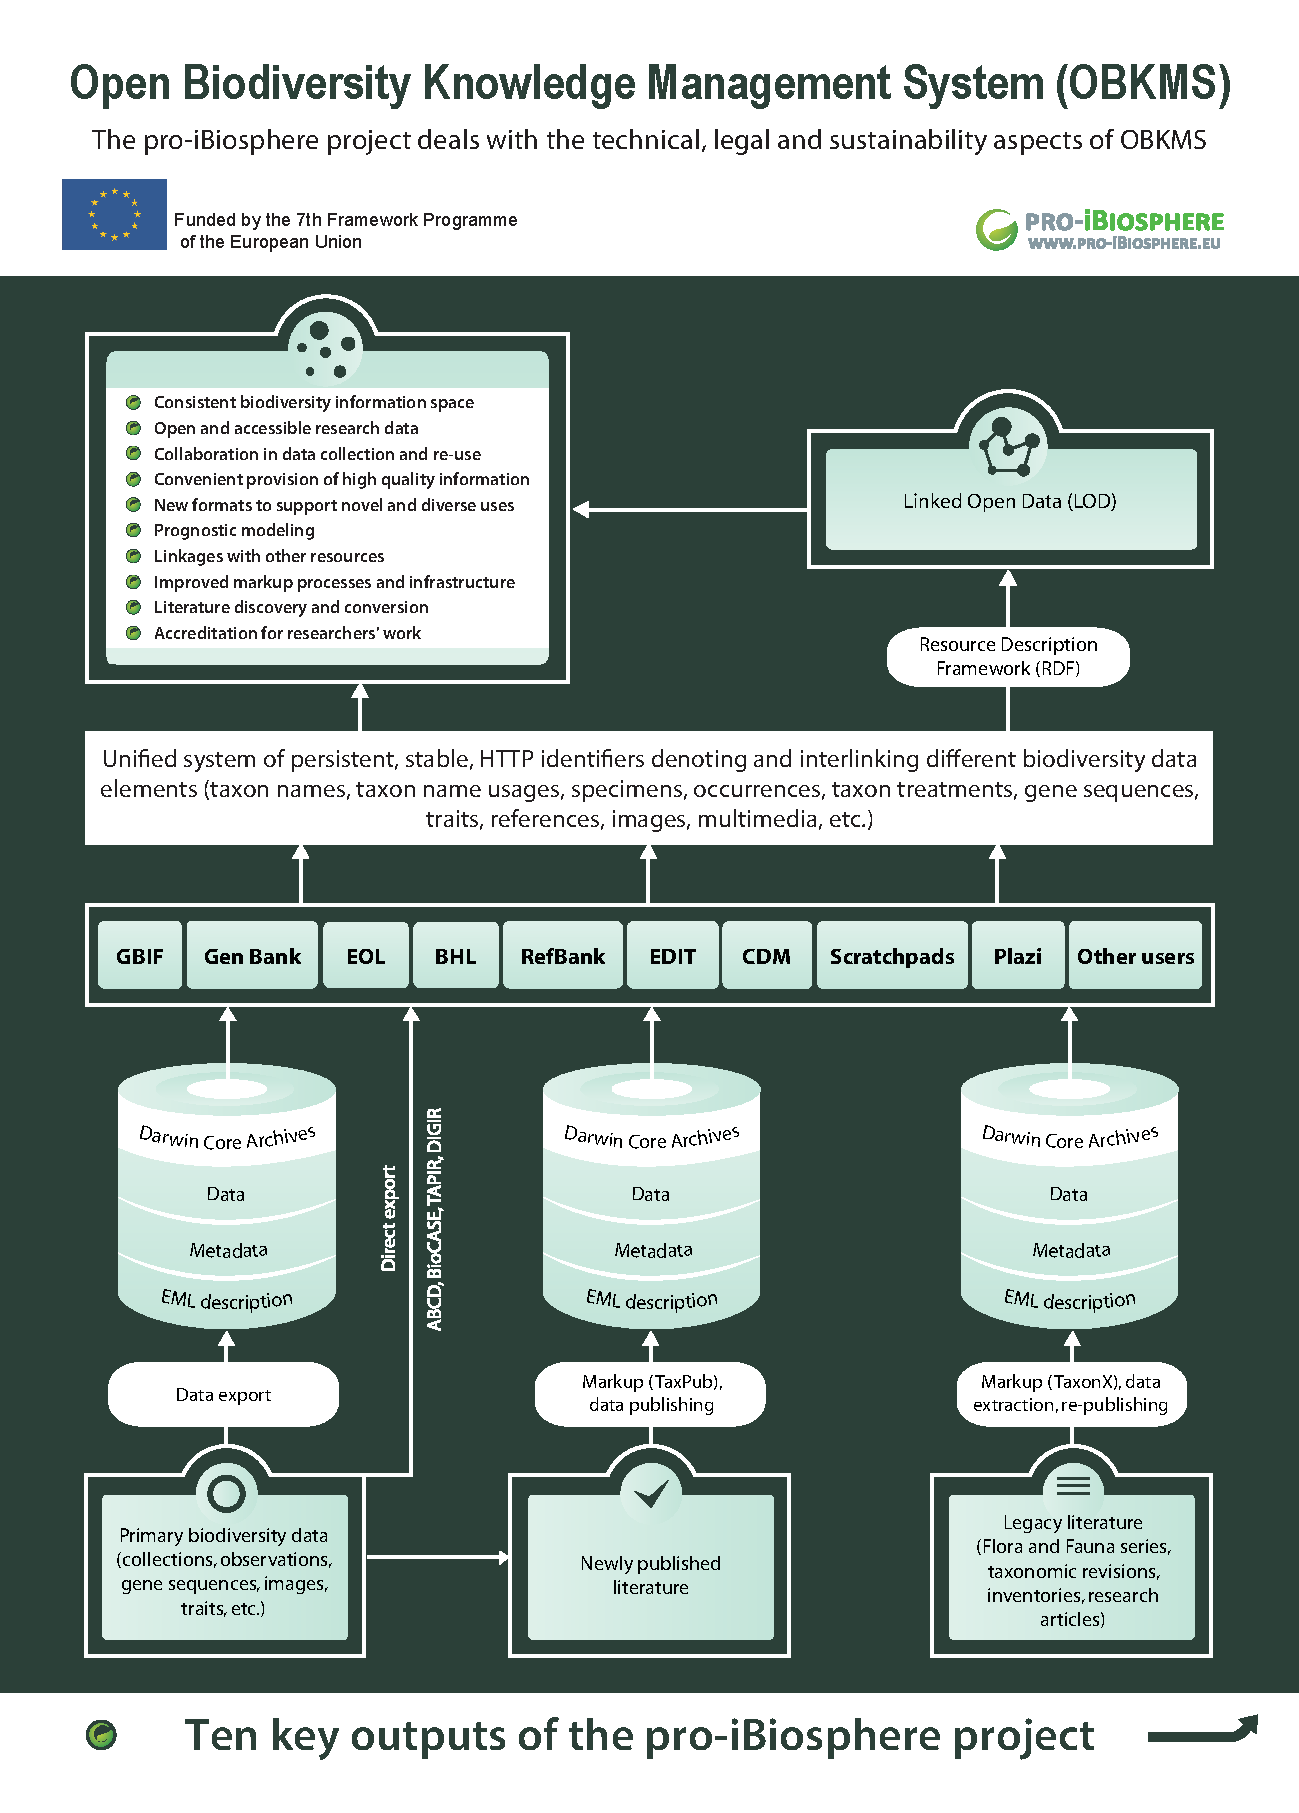
\includepdf[pages=1]{Figures/OBKMS-brochure}
}




\begin{frame}{Основни констатации}
\begin{enumerate}

\item{Различни видове данни: таксономични, биогеографски, филогенетични, визуални, описателни и др.}

\item{Съхранявани разпокъсано из мрежата в полу-структуриран вид, но с подходящи лицензи.}

\item{Нужда от универсална система за именуване на таксономичните концепции поради недостатъците на линеевите имена за компютърната таксономия.}

\end{enumerate}
\end{frame}



\begin{frame}{Цел и задачи}

\begin{alertblock}{Цел}
Създаване на отворена система за информация за биоразнообразието, OpenBiodiv, основана на знание, извлечено от научната литература.
\end{alertblock}

\begin{block}{Задачи}
\begin{enumerate}

\item{Софтуерна архитектура} 

\item{Онтология на областта}

\item{Свързани отворени данни}

\item{Съпътвсваща софтуерна библиотека}

\item{Разработване на работни процеси}

\item{Уеб портал} 

\end{enumerate}
\end{block}
\end{frame}

%---------------------------------------------------------
%Highlighting text
\begin{frame}{Методология}

\begin{enumerate}
\item {Семантичен граф (RDF triple store) като база от знания}
\item{Източници на информация: XML-базирани научни статии; интеграция посредством таксономичния гръбнак, публикуван от института GBIF}
\item{R среда за програмиране, SPARQL като език за запитване}

\end{enumerate}

\end{frame}
%---------------------------------------------------------

\begin{frame}{Резултати}

\begin{enumerate}
    \item Софтуерна архитектура на OpenBiodiv (глава~1 и \cite{senderov_open_2016}).
    \item Концептуализация на областта на публикуването на знание за биоразнообразието във вид на онтологията OpenBiodiv-O (глава~2 и \cite{senderov_openbiodiv-o:_2018}). 
    \item Свързани отворени данни OpenBiodiv-LOD, под формата на RDF, обединяващи таксономично знание от Пенсофт, Плаци и GBIF (глава~3).
    \item Софтуерен пакет за манипулиране на RDF в средата за програмиране R, RDF4R (глава~4).
    \item Работен процес за автоматично вмъкване в онлайн ръкопис на данни от BOLD, GBIF, iDigBio, PlutoF. Автоматично създаване на онлайн ръкопис от EML файл с метаданни (глава~5 и \cite{senderov_online_2016}).
    \item Уеб сайт \href{http://openbiodiv.net}{openbiodiv.net} (глава~6).

\end{enumerate}
    
\end{frame}

\section{Архитектура на OpenBiodiv}
%---------------------------------------------------------
%Two columns
\begin{frame}
\frametitle{Семантични графове (пр. GraphDB) vs. графове (пр. Neo4J)}
\begin{columns}
\column{0.5\textwidth}
\centering
Семантичен граф (пр. GraphDB)
\\
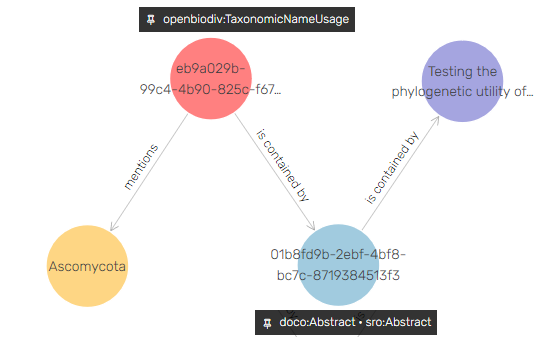
\includegraphics[height = 4cm, width=\textwidth]{Figures/tnu-vis}

\column{0.5\textwidth}
\centering
Граф (пр. Neo4j)
\\
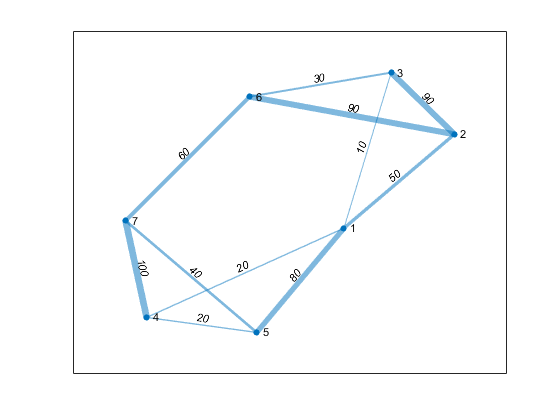
\includegraphics[height = 4cm, width=\textwidth]{Figures/labeled-graph}
\end{columns}
\end{frame}
%---------------------------------------------------------


\begin{frame}{Семантични графове (пр. GraphDB) vs. графове (пр. Neo4J)}

\adjustbox{max width=\textwidth}{
\begin{tabular}{p{3cm}p{6cm}p{6cm}}

Критерий   & Семантичен граф & Граф\\
\hline
Семантика & В самата база данни като OWL или RDFS-изрази. Единно пространство за данни. Изисква експертни онтолози да извличат знания. & Формална семантика обикновено липсва. Бързо внедряване. Унифицирано пространство за данни по-трудно постижимо. \\
\hline
Извод & От самата база данни чрез онтологията или посредством SPARQL. С общо предназначение, по-бавен. & Външен за базата данни. Трябва да се напише за всяка конкретна задача. Със специално предназначение. По-бърз. \\
\hline
Общност & Богата и зряла общност от онтолози и инженери по знания. Много онтологии за различните дисциплини. Стремяща се към стандарти. & Моделите се създават ad-hoc от програмисти за дадена задача. Постигането на интер-оперативност на данните изисква усилия. Стремяща се към работещи приложения. \\
\hline
\end{tabular}
}

    
\end{frame}



\begin{frame}{Компоненти на OpenBiodiv}
\centering
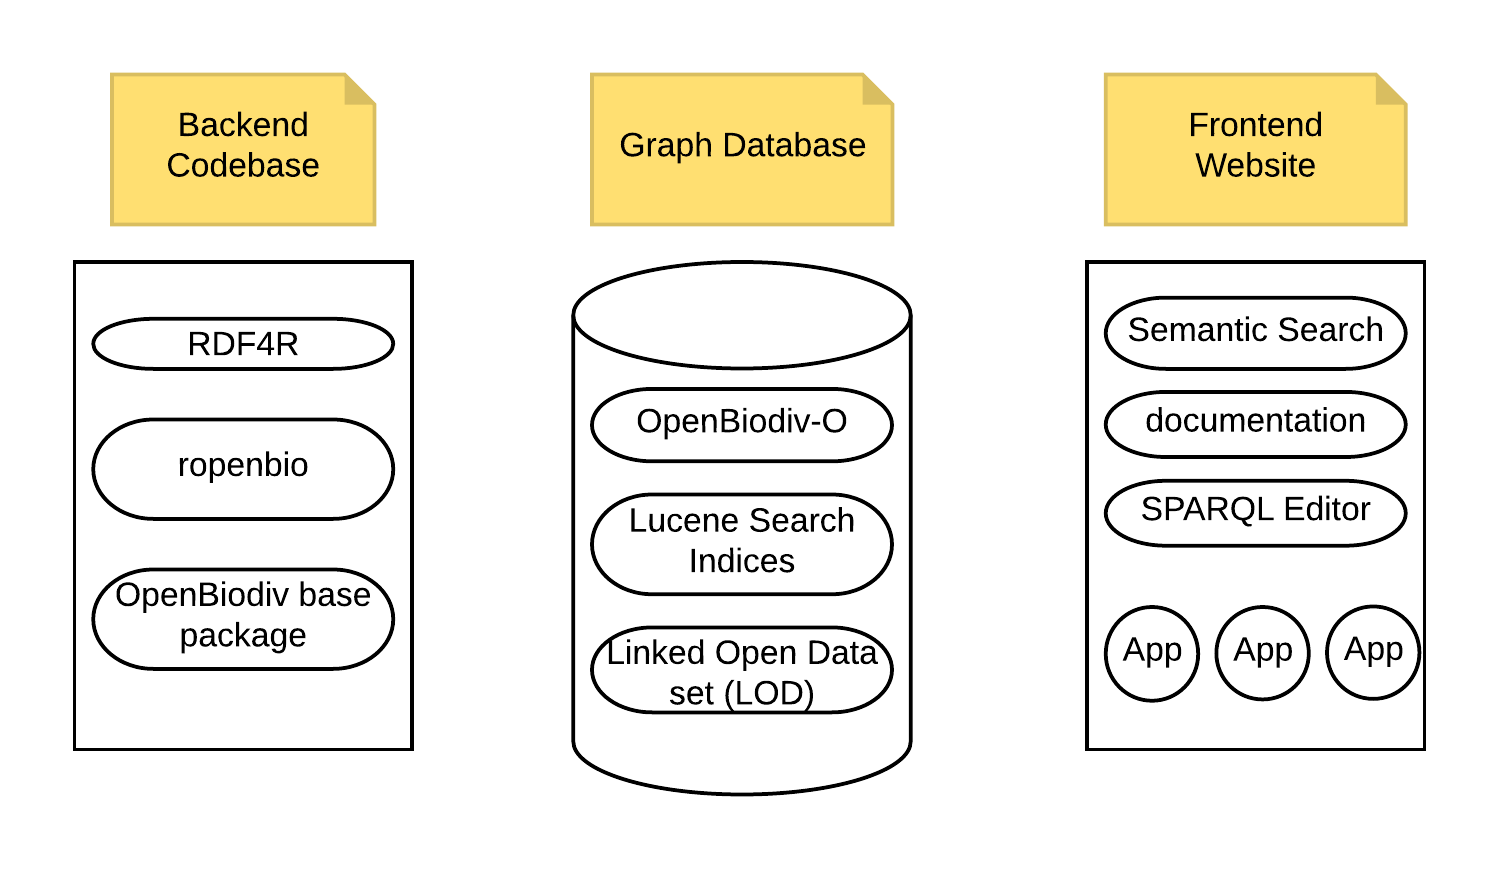
\includegraphics[width=\textwidth]{Figures/components-openbiodiv}
\decoRule

\end{frame}

\begin{frame}{Поток на информацията}
\centering
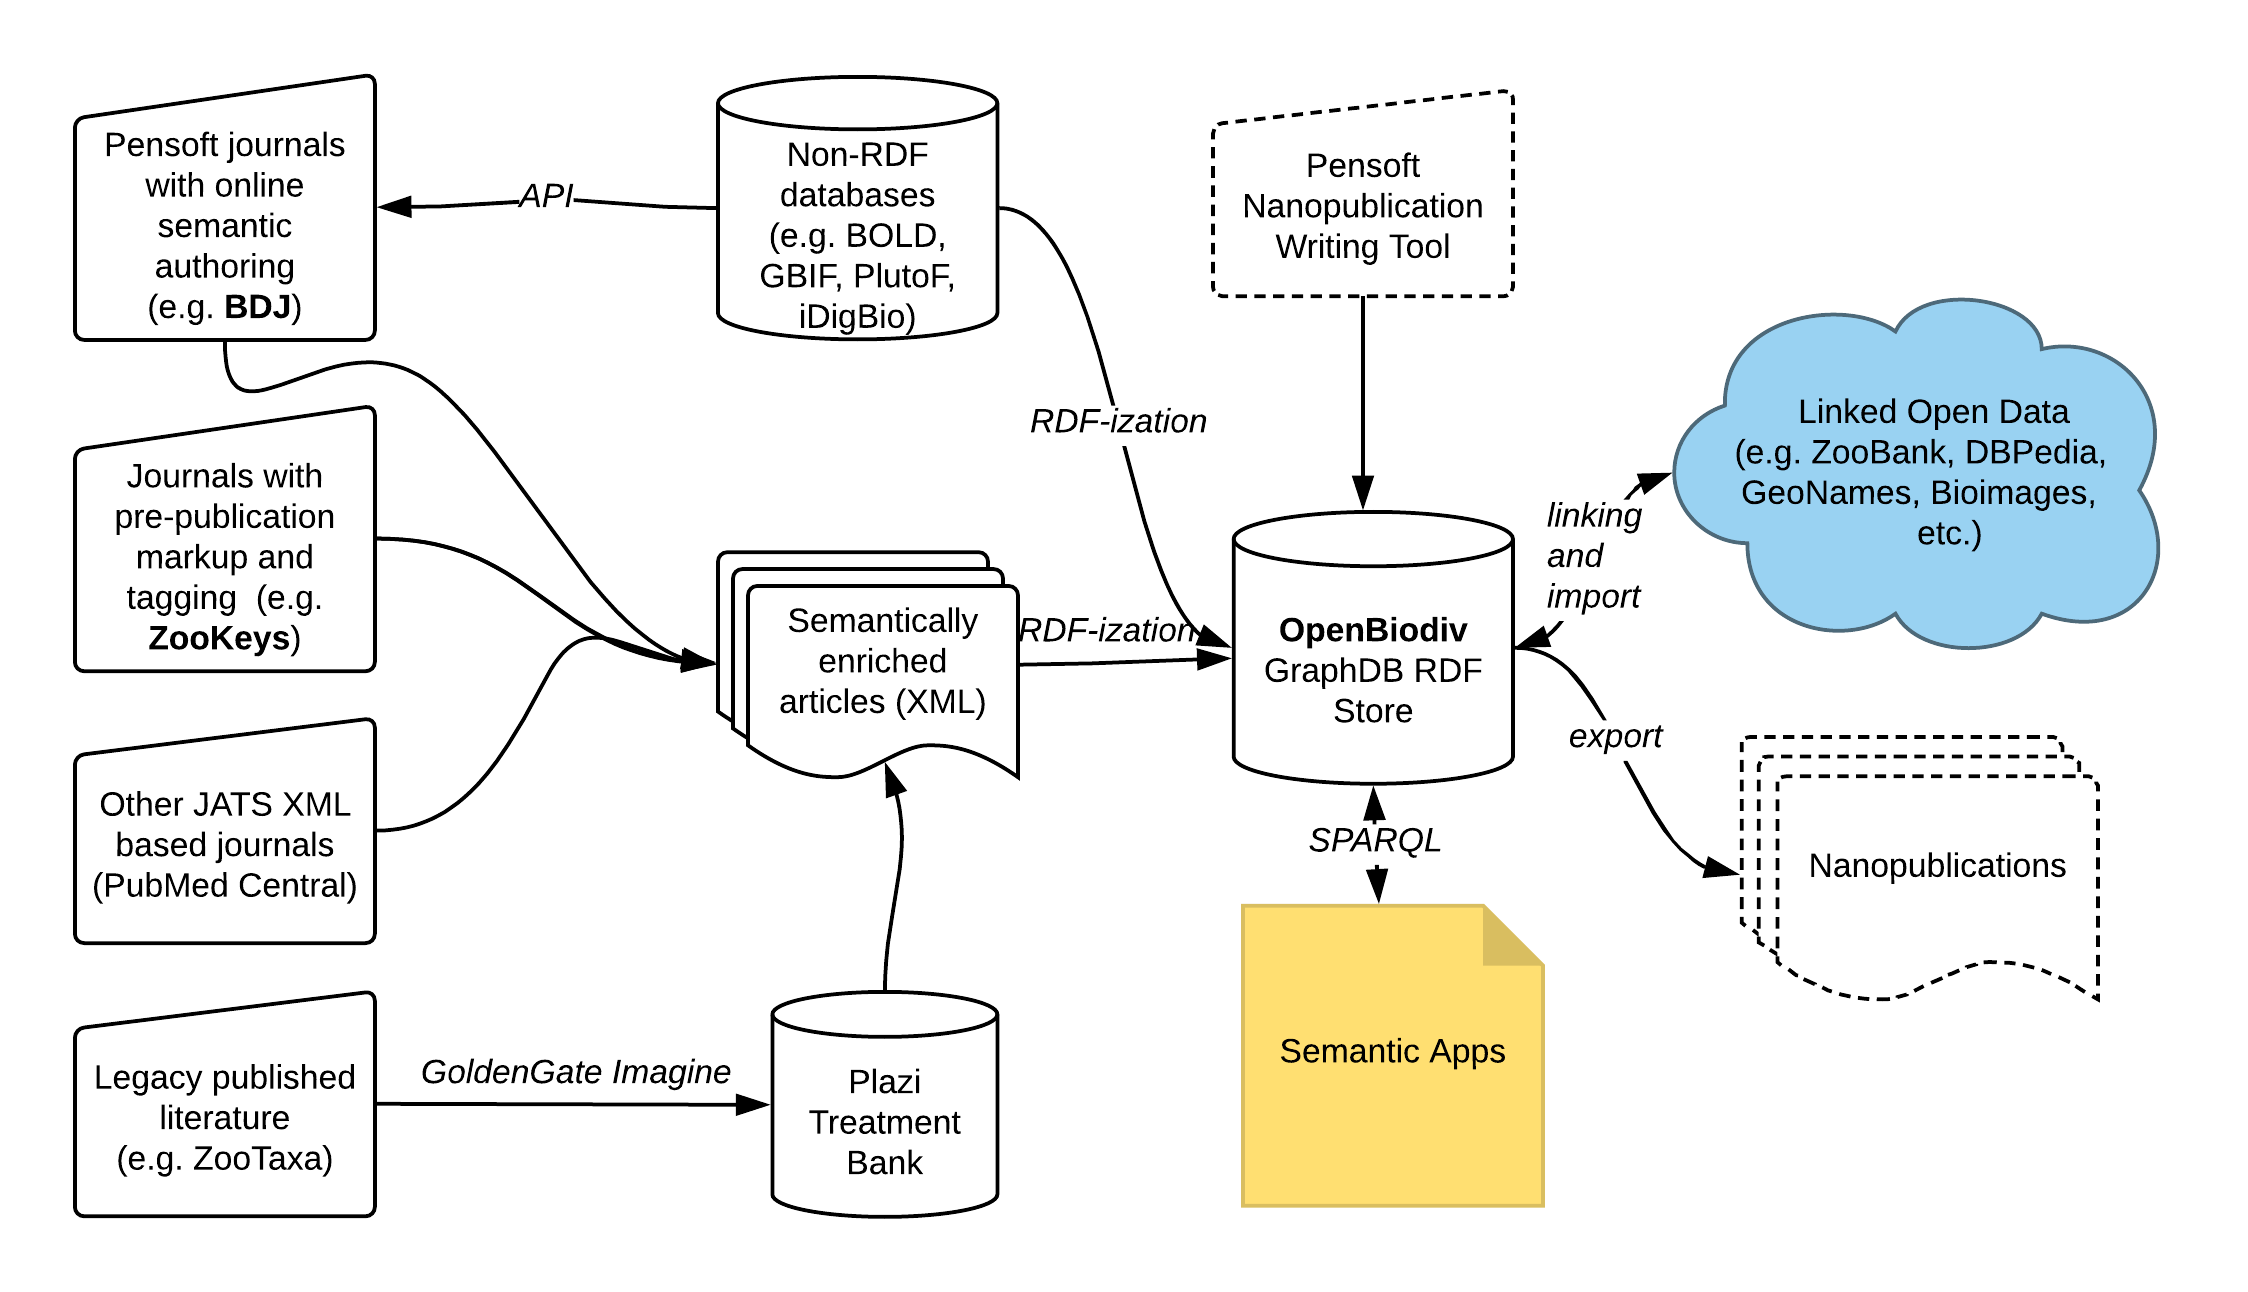
\includegraphics[width=\textwidth]{Figures/openbiodiv-sources}
\decoRule

\end{frame}

\begin{frame}{Поток на информацията}
\centering
\adjustbox{max height=8cm, max width=\textwidth}{
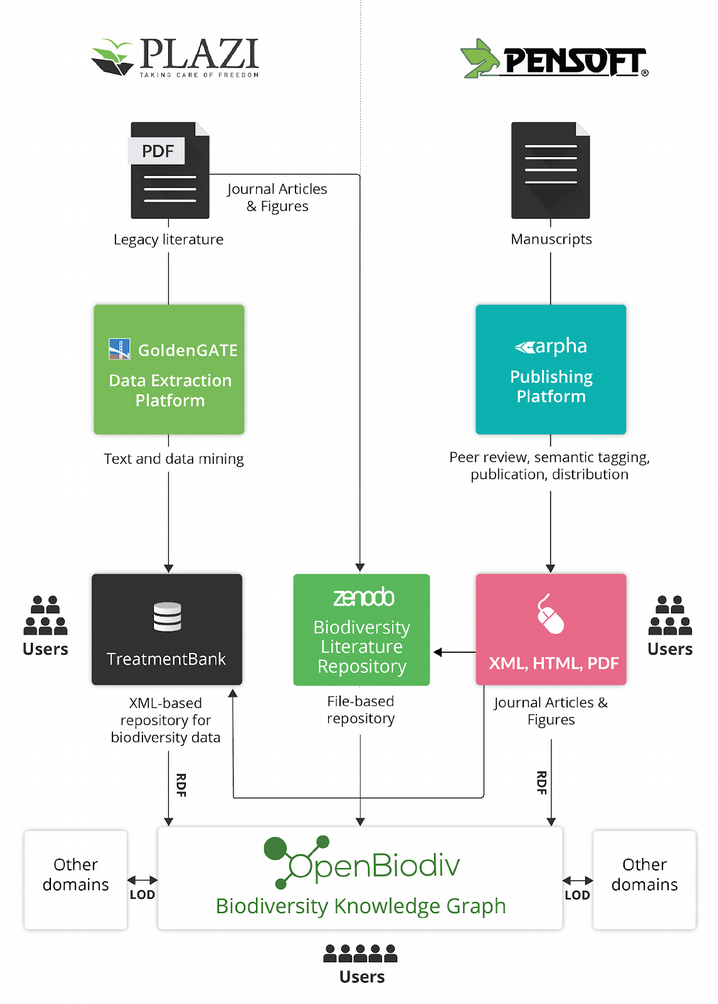
\includegraphics[height=8cm]{Figures/new-workflow}

}

\end{frame}



\section{Oнтология на OpenBiodiv}

\begin{frame}{OpenBiodiv-O}
\begin{enumerate}
    \item Концептуализация на областта
    \item Семантично моделиране на домейна за публикуване на знание за биоразнообразието
    \item Семантично моделиране на биологичната номенклатура
    \item Семантично моделиране на таксономичните концепции
\end{enumerate}
\end{frame}

\begin{frame}{Нови класове в областта на публикуването на знание за биоразнообразието}

      \begin{tabular}{cc}
        \hline
          Class QName             & Comment\\  \hline
  {\tt :Treatment}                & section of a taxonomic article\\
  {\tt :NomenclatureSection}      & subsection of Treatment\\
  {\tt :NomenclatureHeading}      & contains a nomenclatural act \\
  {\tt :NomenclatureCitationList} & list of citations of related concepts\\
  {\tt :MaterialsExamined}        & list of examined specimens\\
  {\tt :BiologySection}           & subsection of Treatment\\
  {\tt :DescriptionSection}       & subsection of Treatment\\
  {\tt :TaxonomicKey}             & section with an identification key\\
  {\tt :TaxonomicChecklist}       & section with a list of taxa for a region\\ 
  {\tt :TaxonomicNameUsage}       & mention of a taxonomic name\\ \hline

      \end{tabular}
      
\end{frame}


\begin{frame}{Превод в RDF на таксономична статия}
\centering
\adjustbox{max height=8.5cm}{
	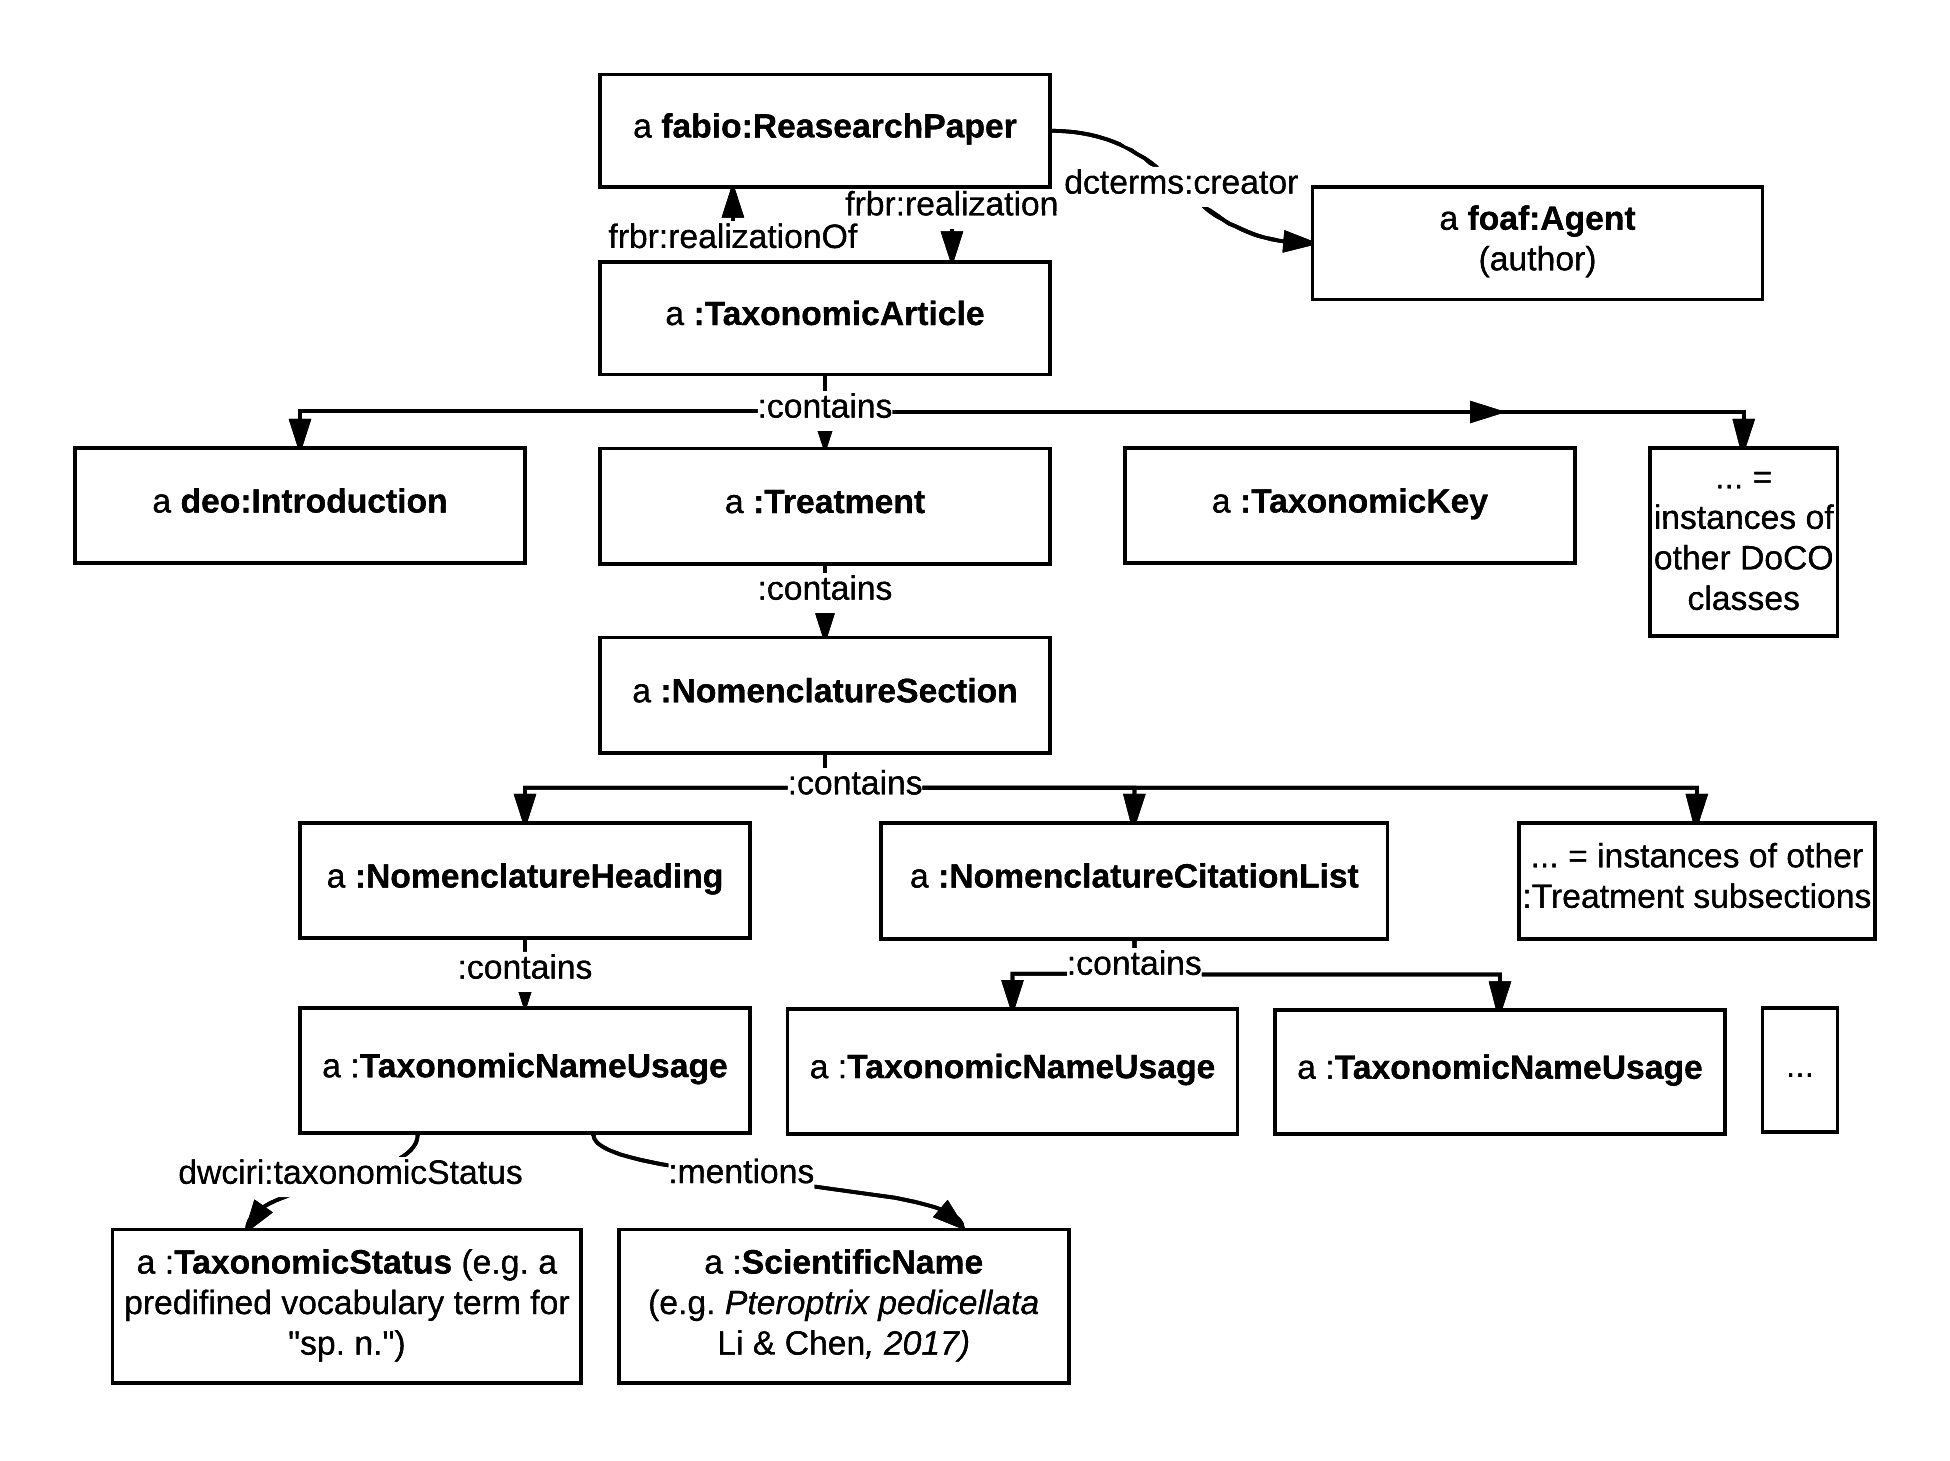
\includegraphics[width=\textwidth]{Figures/taxonomic-article-diagram}
	\decoRule}
	
  
\end{frame}


\begin{frame}{Моделиране на таксономичната номенклатура}
  \centering
  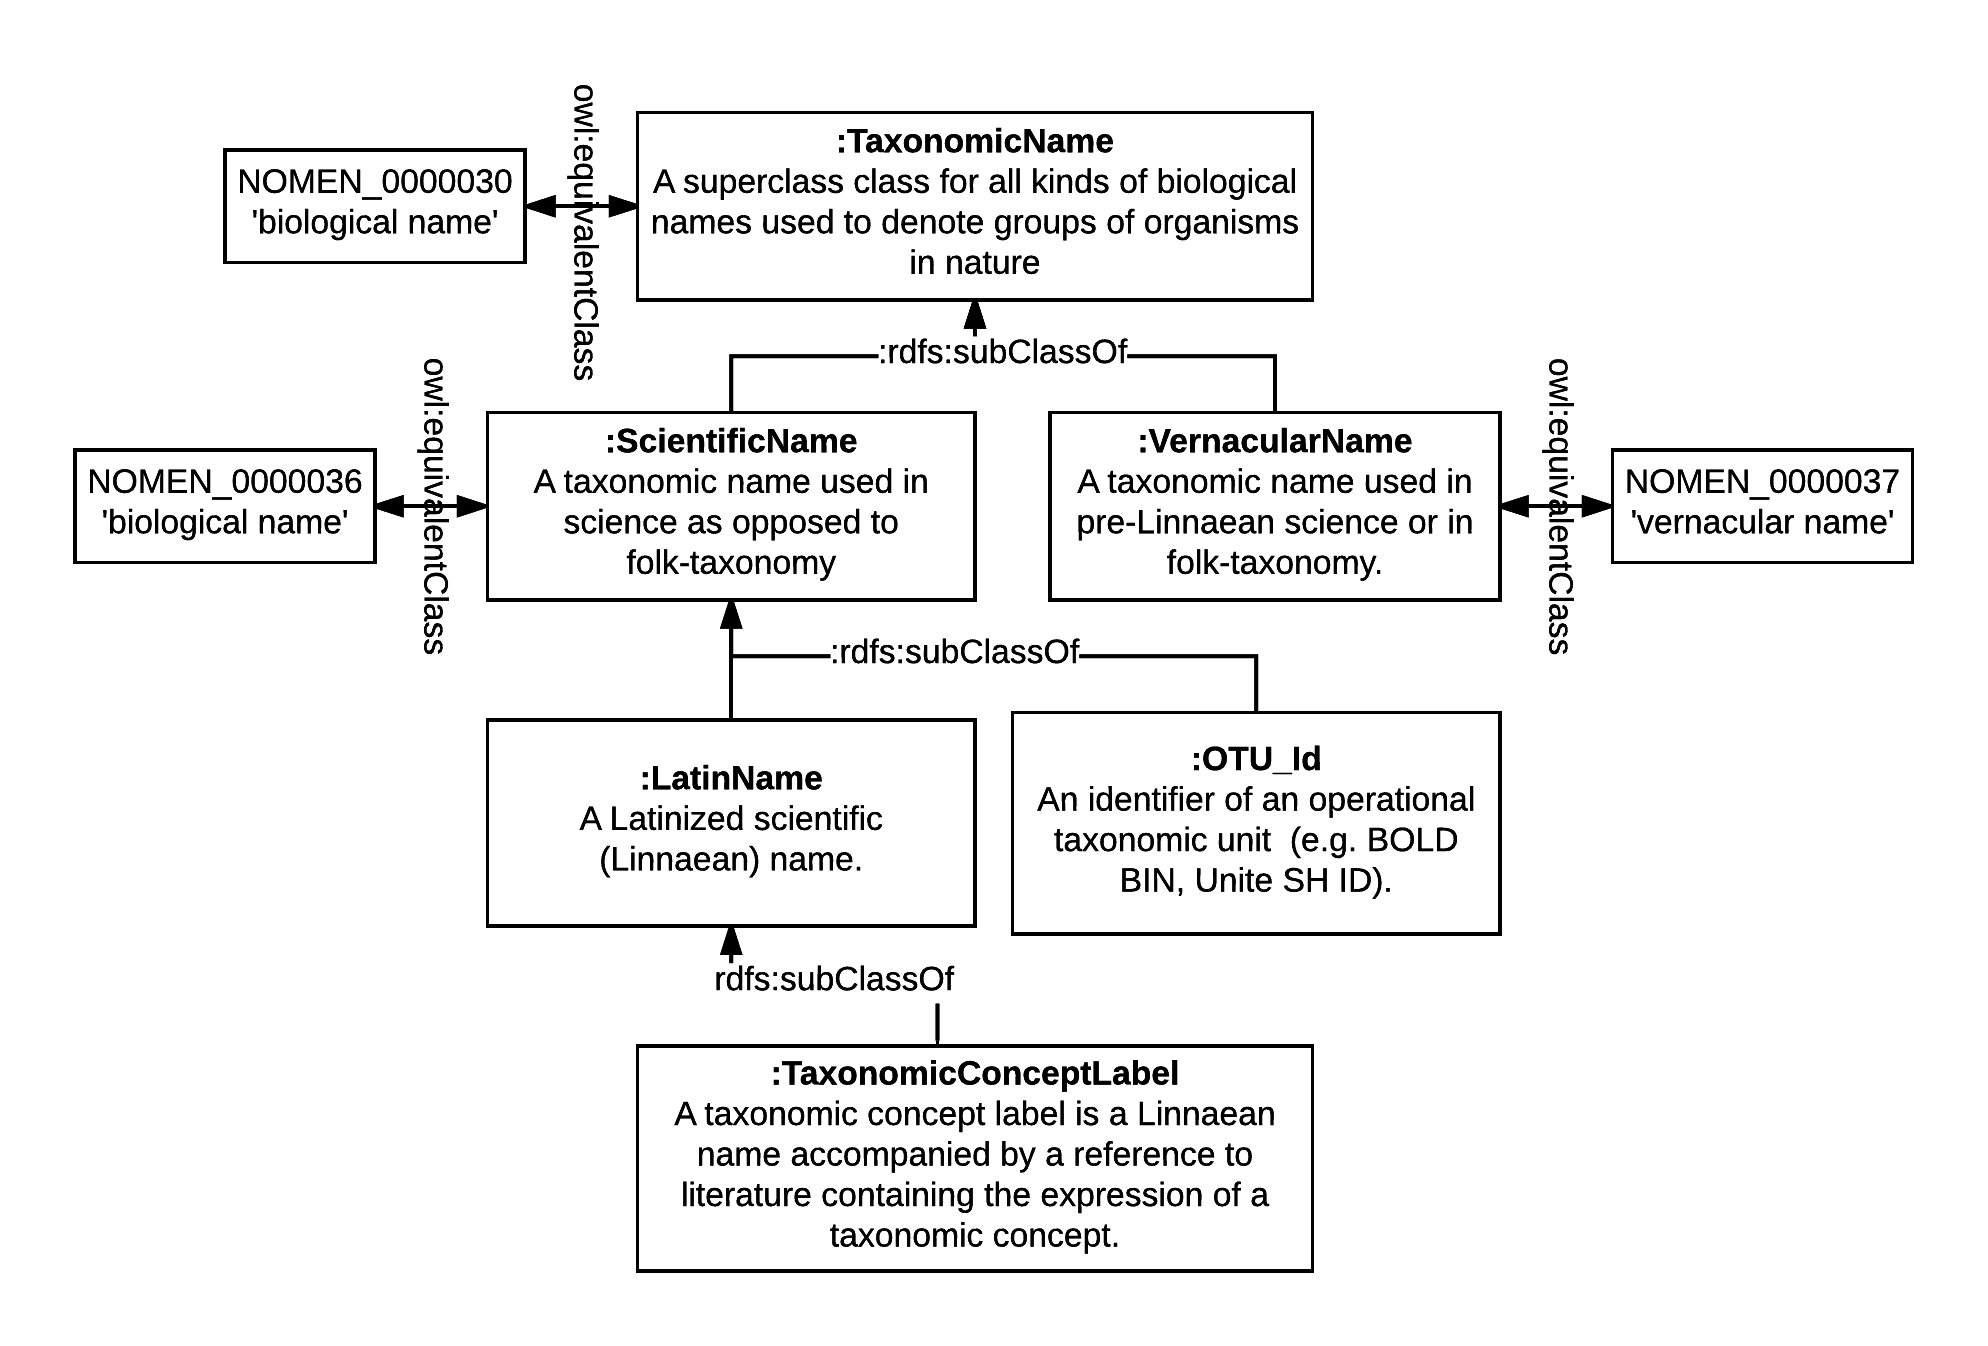
\includegraphics[width=\textwidth]{Figures/taxonomic-name-class-hierarchy-diagram}
  \decoRule
  
\end{frame}



\begin{frame}{Речник с таксономични термини.}
\adjustbox{max width=\textwidth}{\begin{tabular}{ccc}
\hline
Vocabulary Instance QName & Example Abbrev & Comment\\ \hline
{\tt :TaxonomicUncertainty} & \emph{incertae sedis} & Taxonomic Uncertainty\\
{\tt :TaxonDiscovery} & \emph{sp. n.} & Taxonomic Discovery \\
{\tt :ReplacementName} & \emph{comb. n.} & Replacement Name \\
{\tt :UnavailableName} & \emph{nomen dubium} &  Unavailable Name \\
{\tt :AvailableName} & \emph{stat. rev.} & Available Name \\
{\tt :TypeSpecimenDesignation} & \emph{lectotype designation} & Type Specimen Designation \\
{\tt :TypeSpeciesDesignation} & \emph{type species} & Type Species Designation\\
{\tt :NewOccurrenceRecord} & \emph{new country record} & New Occurrence Record (for region)\\
\hline
\end{tabular}
}
\end{frame}


\begin{frame}{Взаимоотношения между имена}
 \centering
  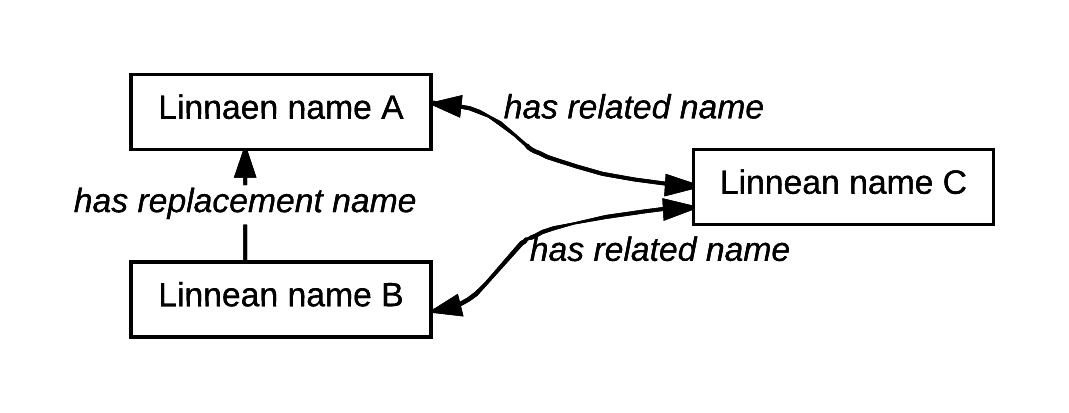
\includegraphics[width=\textwidth]{Figures/scientific-name-patterns}
  \decoRule
  
\end{frame}

{
\setbeamercolor{background canvas}{bg=}
\includepdf[pages=18]{Figures/taxonomy-computers}
}




\begin{frame}{Взаимоотношения между таксономични концепции}

Region Connection Calculus 5
\begin{enumerate}
    \item Equal ==    
    \item Disjoint ~!
    \item Overlap   ><
    \item Proper part  <
    \item Inverse proper part >
\end{enumerate}

\end{frame}


\begin{frame}{Взаимоотношения между таксономични концепции}
\centering
  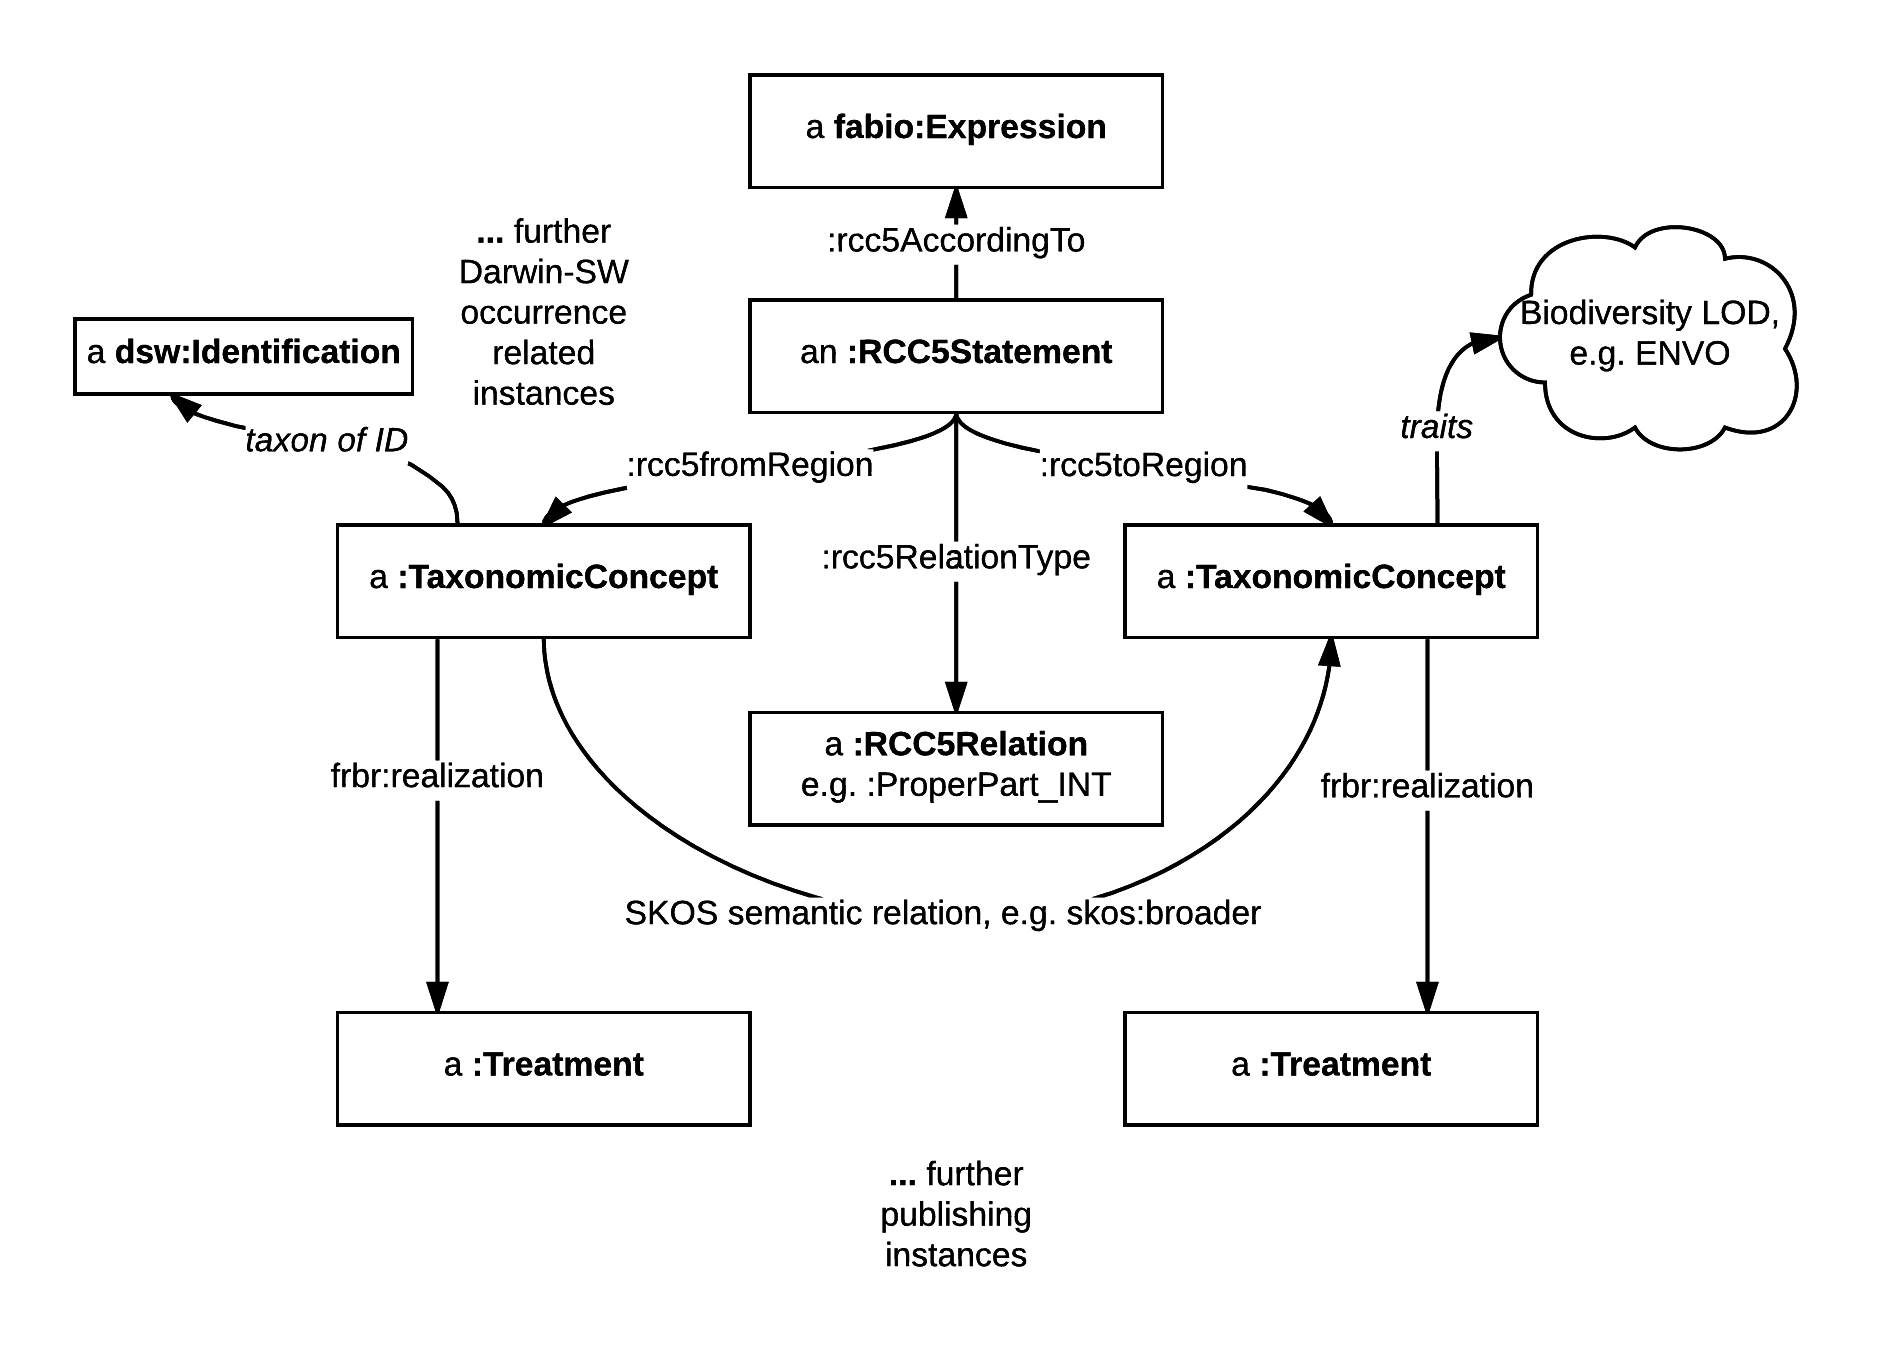
\includegraphics[width=\textwidth]{Figures/taxonomic-concept-relationships-diagram}
  \decoRule
  
\end{frame}

\section{Свързани отворени данни}

\begin{frame}{Избор на източници на информация}
\begin{itemize}
    \item Академични списания на Пенсофт, публикуващи знание за биоразнообразието: ZooKeys, Biodiversity Data Journal и т.н.
    \item База данни с таксономични дискусии (treatment) на Плаци
    \item Таксономичен гръбнак на GBIF за интеграция
\end{itemize}
\end{frame}

\begin{frame}{Списания, чиито статии  са превърнати в RDF}
\adjustbox{max width=\textwidth}{  \begin{tabular}{ccc}
        \hline
          Journal Name             & Submission Style & Number of Articles\\  \hline
          ZooKeys                 & Word document & 3829\\
          PhytoKeys               & Word document & 537\\
          MycoKeys                & Word document & 127\\
          Biodiversity Data Journal & Web based (ARPHA) & 490\\
          Journal of Orthoptera Research & Word document & 32
      \end{tabular}}
    
   
\end{frame}

\begin{frame}{Типове данни, маркирани в TaxPub and TaxonX и тяхната кореспондеция към RDF}

\adjustbox{max width=\textwidth}{\begin{tabular}{cccc}
        \hline
          Datatype             & TaxPub & TaxonX & RDF Type\\  \hline
          Article metadata     & T & T & {\tt fabio:JournalArticle} and related\\
          Keyword group        & T & F & {\tt openbiodiv:KeywordGroup} \\
          Abstract             & T & T & {\tt sro:Abstract}\\
          Title                & T & F & {\tt doco:Title} \\
          Author               & T & T & {\tt foaf:Person} \\
          Introduction section & T & F & {\tt deo:Introduction}\\
          Discussion section   & T & T & {\tt orb:Discussion}\\
          Treatment section    & T & T & {\tt openbiodiv:Treatment}\\
          Nomenclature section & T & T & {\tt openbiodiv:NomenclatureSection}\\
          Materials examined   & T & T & {\tt openbiodiv:MaterialsExamined}\\
          Diagnosis section    & T & T & {\tt openbiodiv:DiagnosisSection} \\
          Distribution section & T & T & {\tt openbiodiv:DistributionSection}\\
          Taxonomic key        & T & T & {\tt openbiodiv:TaxonomicKey}\\
          Figure               & T & T & {\tt doco:Figure}\\
          Taxonomic name usage & T & T & {\tt openbiodiv:TaxonomicNameUsage}
      \end{tabular}
     }
      
\end{frame}


\begin{frame}{Брой твърдения}
\centering
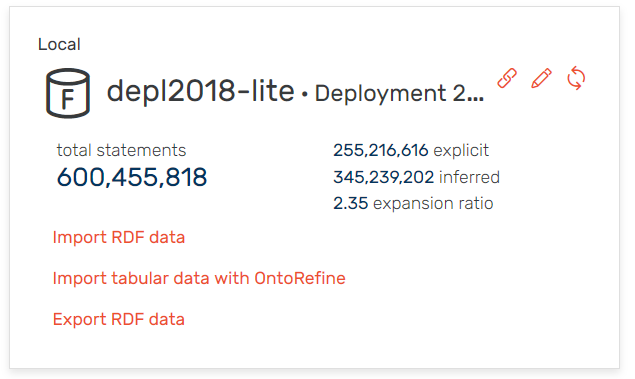
\includegraphics[width=\textwidth]{Figures/active-repository}
\decoRule
\label{fig:statements-report}
\end{frame}


\begin{frame}{Екстрактор}

\begin{algorithmic}[1]
\Procedure {Extractor}{XML Node $X$}
\State $a \leftarrow$ extract atoms of $X$
\Comment Atoms extraction
\State $r \leftarrow$ construct RDF from $a$
\Comment RDF construction
\State $C \leftarrow$ find relevant sub-nodes of $X$
\Comment Recursively applies itself
\State $R \leftarrow$ apply Extractor on each $C_i \in C$
\State \Return $r \bigcup R$
\EndProcedure
\end{algorithmic}
\label{algo:extractor}

\end{frame}


\begin{frame}{Деградацията на производителността при импорт}
\centering
\adjustbox{max width=\textwidth, max height=8cm}{
    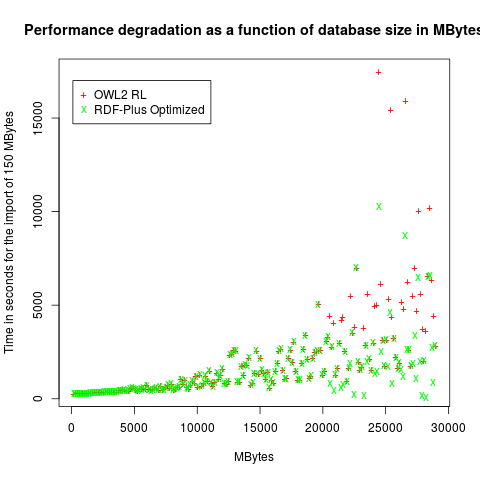
\includegraphics[]{Figures/performance-degradation-both}
    \decoRule
}
\end{frame}


\begin{frame}{Употреба на OpenBiodiv-LOD}
\begin{itemize}
    \item Прости заявки
    \begin{itemize}
        \item Запитване за автор, таксономично име, таксономична концепция, списание и пр.
        \item Запитвания, използващи структурата на статията и таксономичния гръбнак на GBIF
        \item Размито търсене с Lucene
    \end{itemize}
    \item Експертни заявки
    \begin{itemize}
        \item Проверка на валидността на таксономично име
        \item Оценка на научната загуба след пожара в Museu Nacional в Бразилия
    \end{itemize}
\end{itemize}
\end{frame}


\begin{frame}{Museu Nacional}

\lstinputlisting[language=SPARQL,
label=listing:museu-nacional, basicstyle=\ttfamily\tiny]{Listings/museu-nacional-short.txt}

\end{frame}

\begin{frame}{Museu Nacional}
\begin{itemize}
    \item 195 споменавания на MNRJ
    \item в 22 статии на Pensoft
    \item 6 127 различни имена в статиите, които се позовават на материали от MNRJ
    \begin{itemize}
     \item насекоми (Xestoblatta, Charinus, Lamproclasiopa, etc.)
    \item  нематоди (Paracamallanus, Cucullanus, Pseudascarophis, etc.)
    \item  птици (Ichthyouris)
    \item  риби (Sphoeroides)
    \end{itemize}
     
\end{itemize}

\end{frame}

\section{Софтуерни библиотеки}

\begin{frame}{RDF4R}

\begin{enumerate}
    \item Връзка със семантична база данни
    \item Функции за преобразуване на SPARQL заявки в R функции
    \item Работа с литерали и идентификатори
    \item Работа с префикси
    \item Създаване и сериализация на RDF
    \item Основна терминология на семантични понятия
\end{enumerate}
\end{frame}

\begin{frame}{Превръщане на SPARQL заявка в R функция}

\tt
> genus\_lookup <- rdf4r::query\_factory(p\_query = p\_query, access\_options = openbiodiv)\\
> genus\_lookup("Drosophila")\\
#    genus title\\
# 1   Drosophila  Characterisation of the chemical\\
# morphotypes belonging to the Anastrephafraterculus complex\\
# 2   Drosophila                A new species group in the genus Dichaetophora,\\
# descriptions of six new species from the Oriental region (Diptera, Drosophilidae)
\end{frame}

\section{Уеб апликации}

\begin{frame}{Работен поток}
\centering
\adjustbox{max height=10cm}{\centering
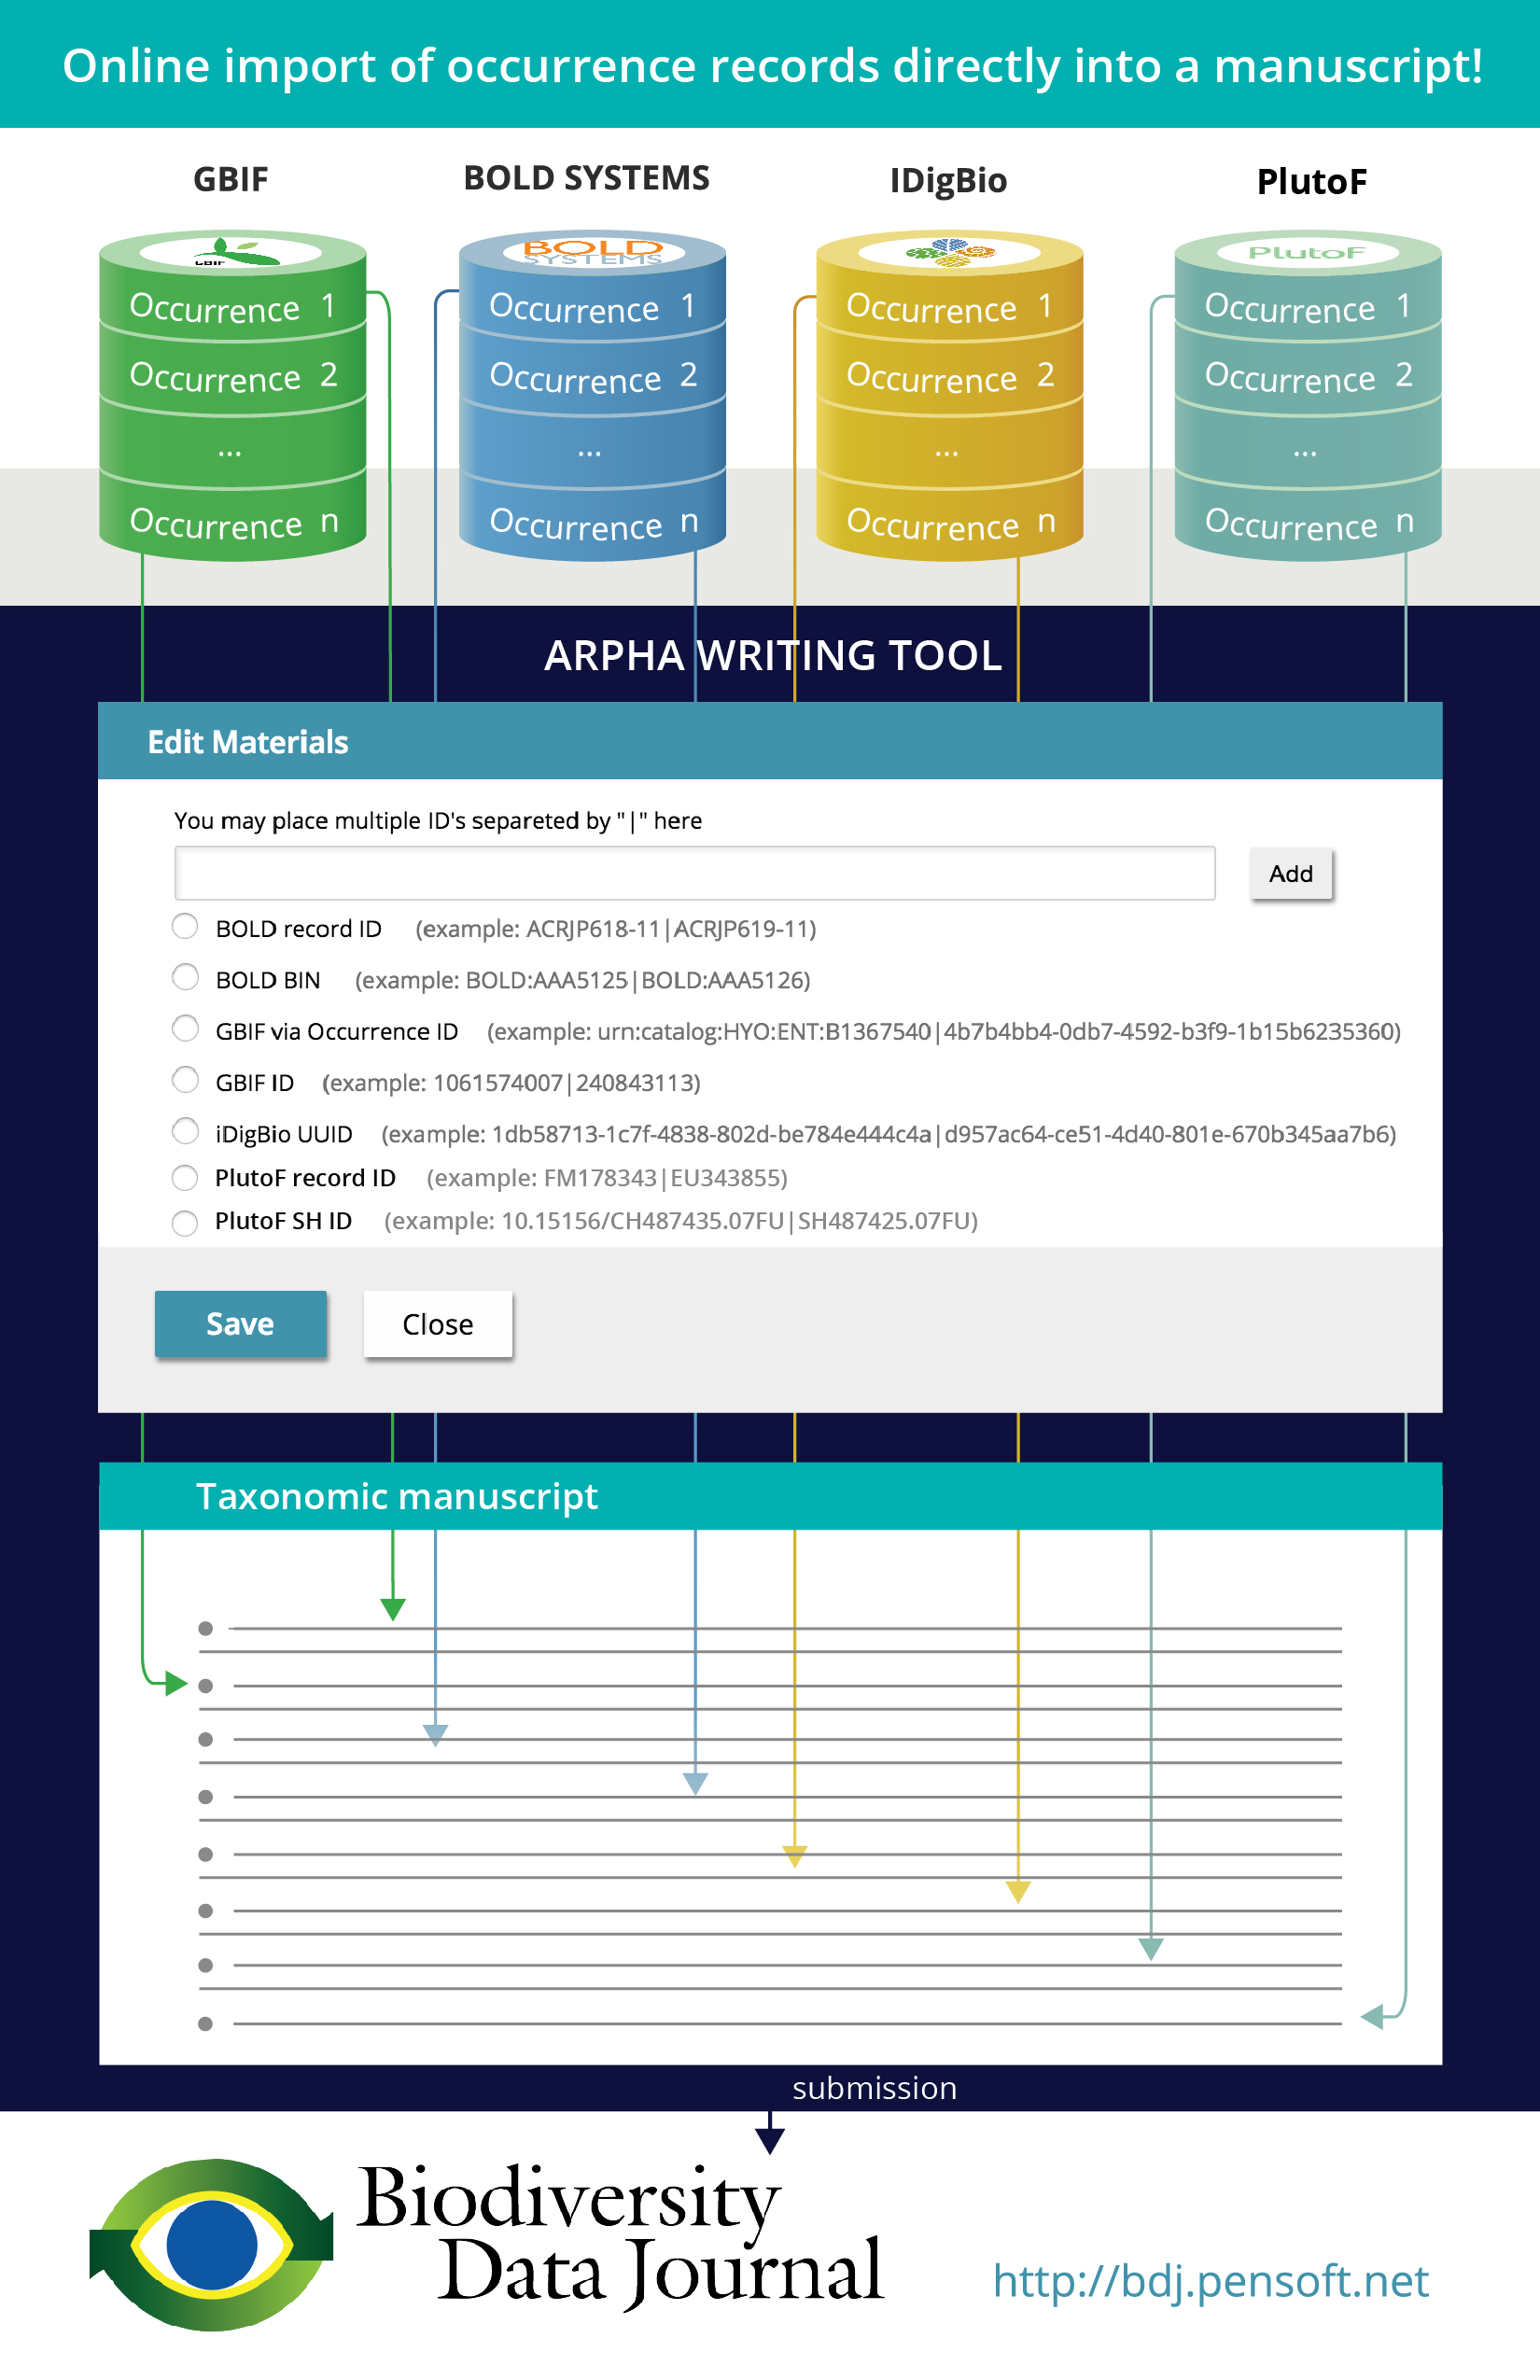
\includegraphics[width=\textwidth]{Figures/workflow-idigbio}
\decoRule

\label{fig:workflow-idigbio}
}

\end{frame}




\begin{frame}{Автоматично създаване на ръкопис}
\centering
\adjustbox{max width=\textwidth}{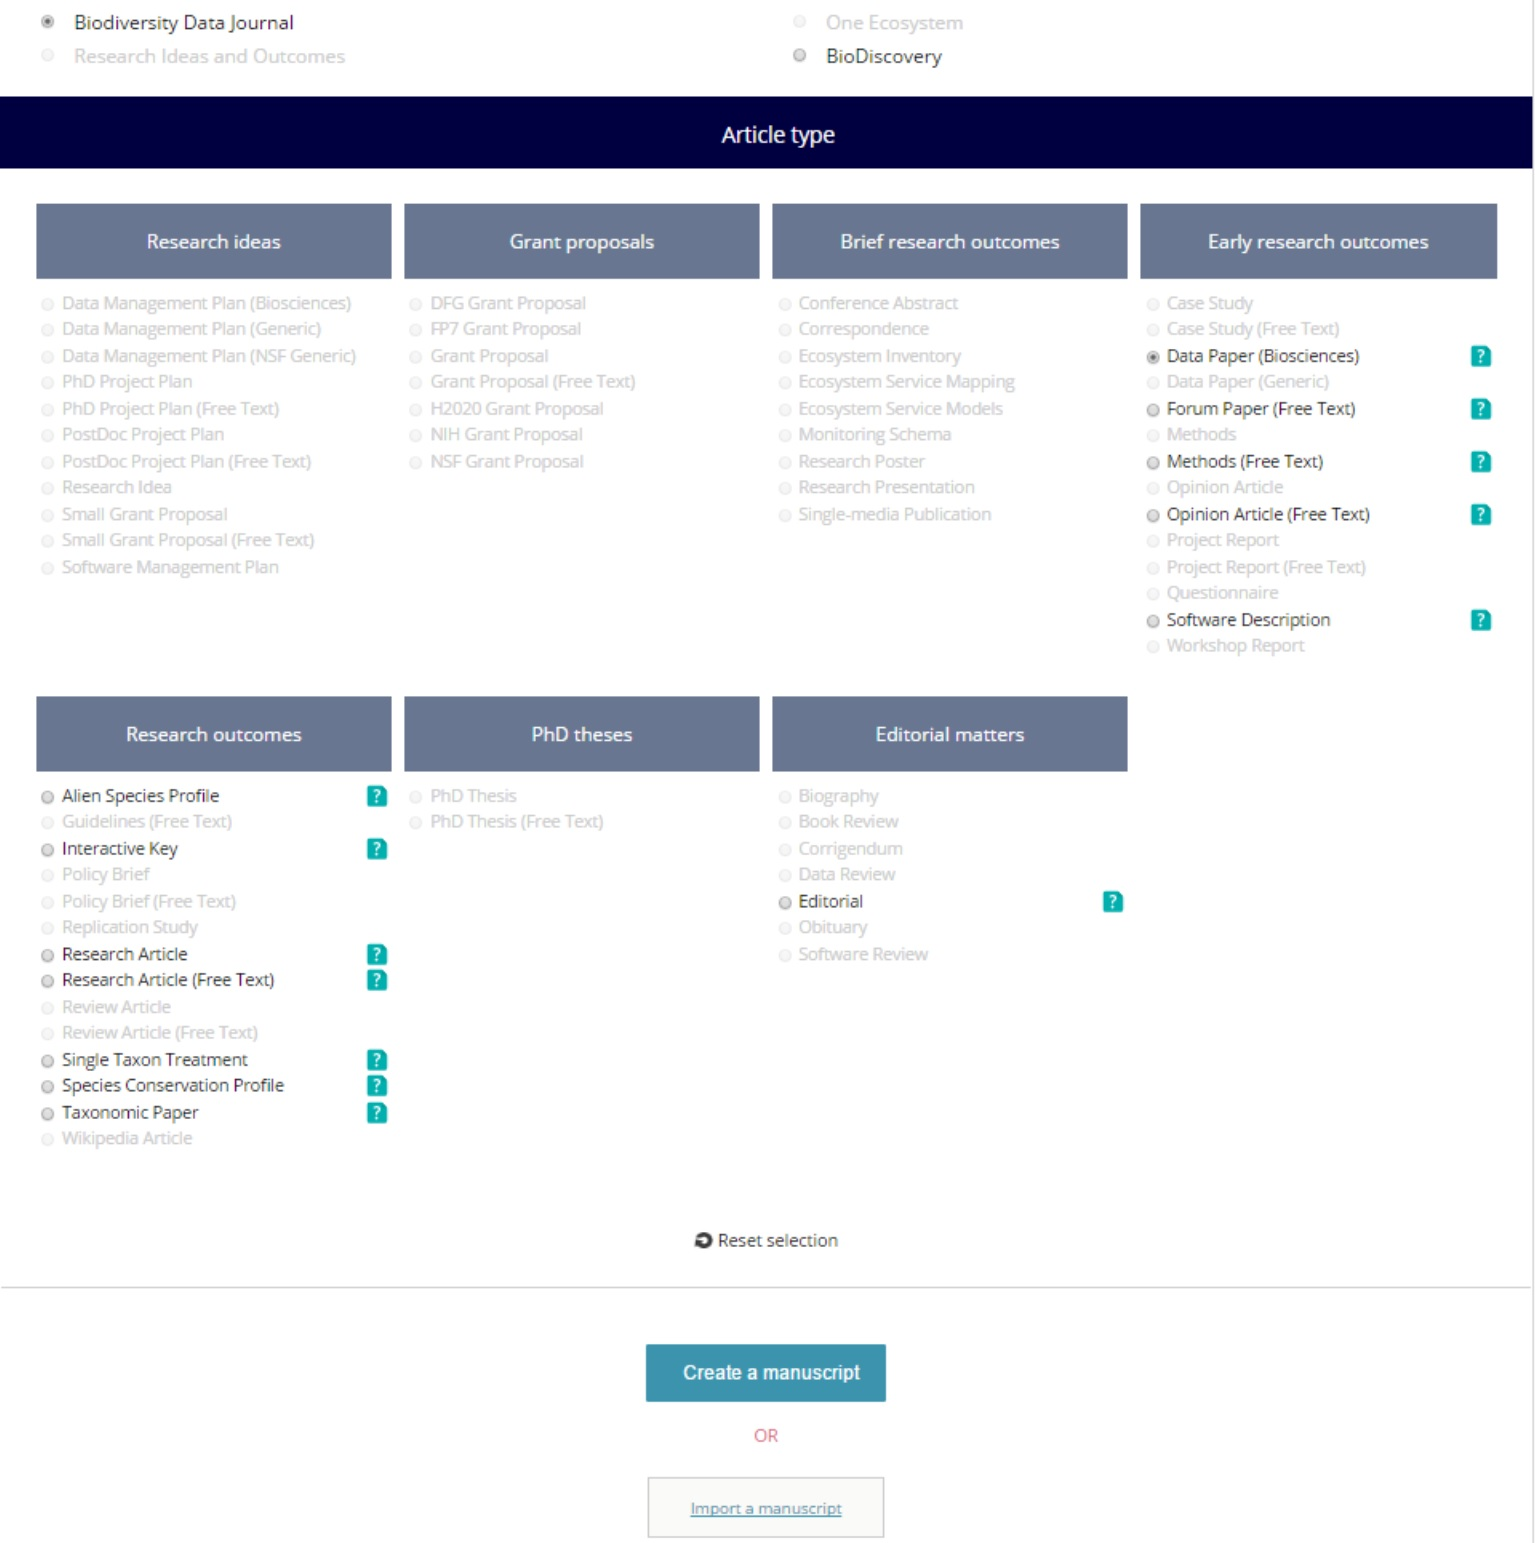
\includegraphics[width=\textwidth]{Figures/journal-selection}
\decoRule
\label{fig:journal-selection}
}
\end{frame}

\begin{frame}{Автоматично създаване на ръкопис 2}
\centering
\adjustbox{max width=\textwidth}{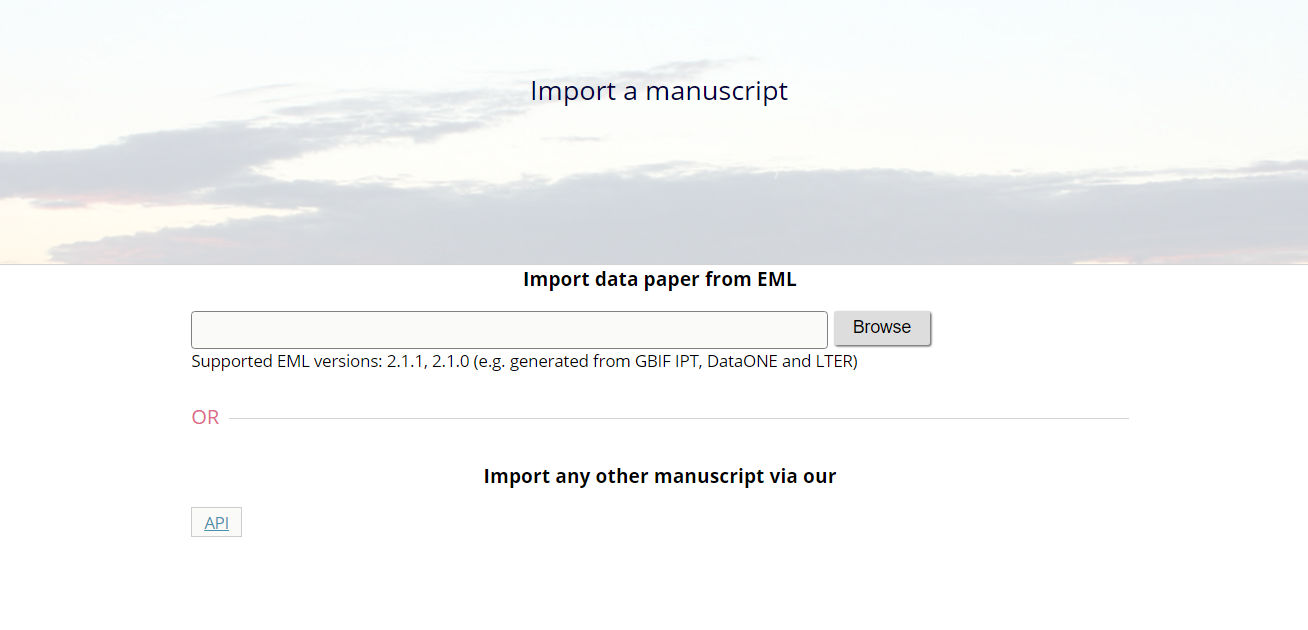
\includegraphics[width=\textwidth]{Figures/user-interface}
\decoRule
\label{fig:user-interface}
}
\end{frame}


{
\setbeamercolor{background canvas}{bg=}
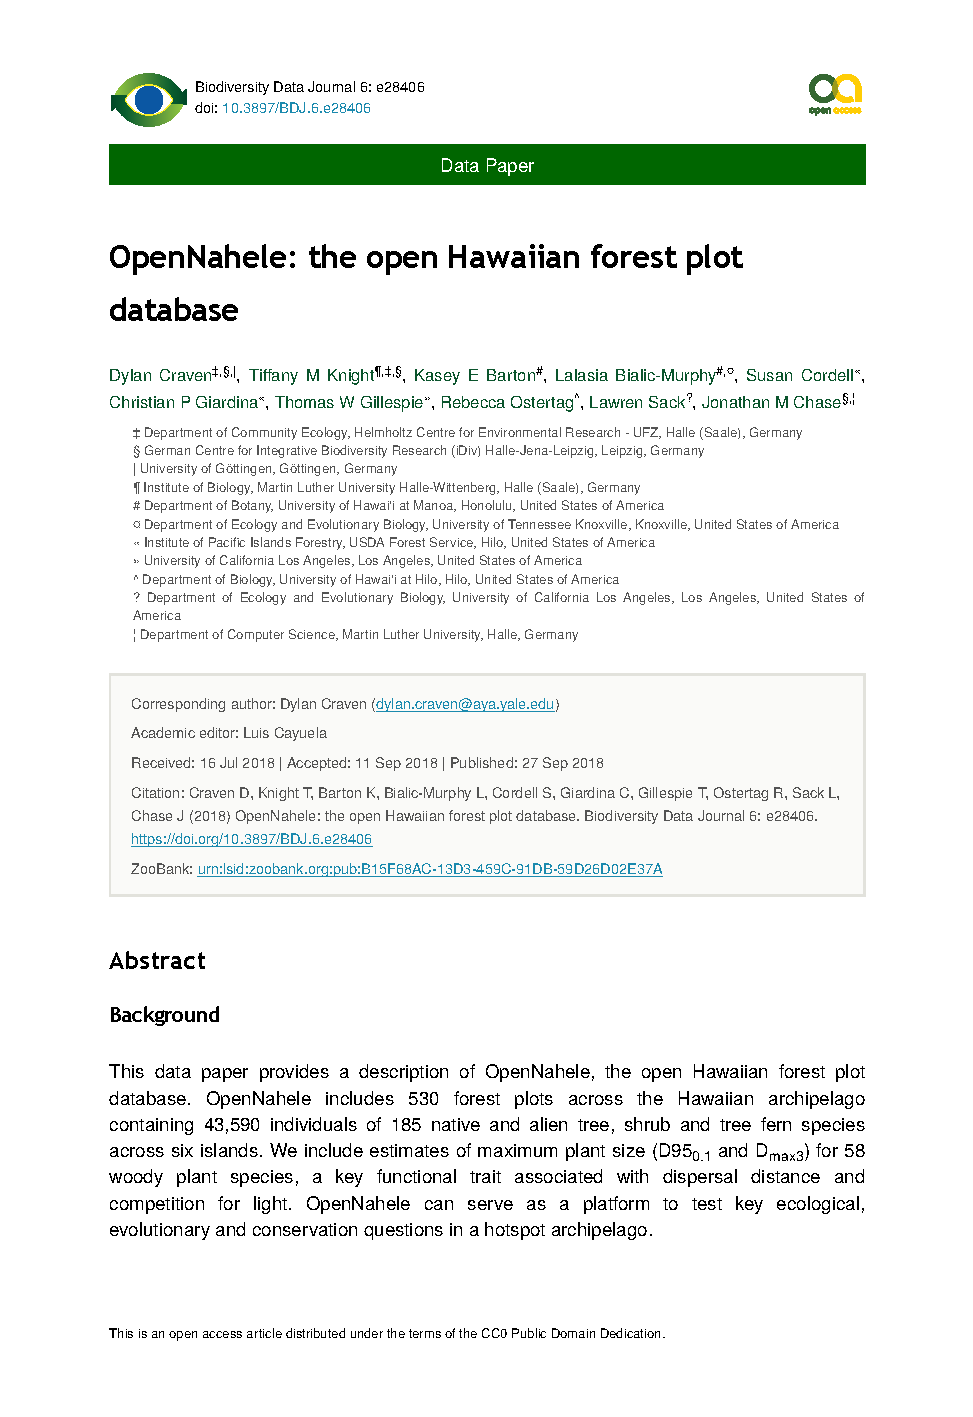
\includepdf[pages=1-2]{Figures/data-paper}
}


\begin{frame}{Уеб портал}
\centering
\adjustbox{max height=9cm}{\centering
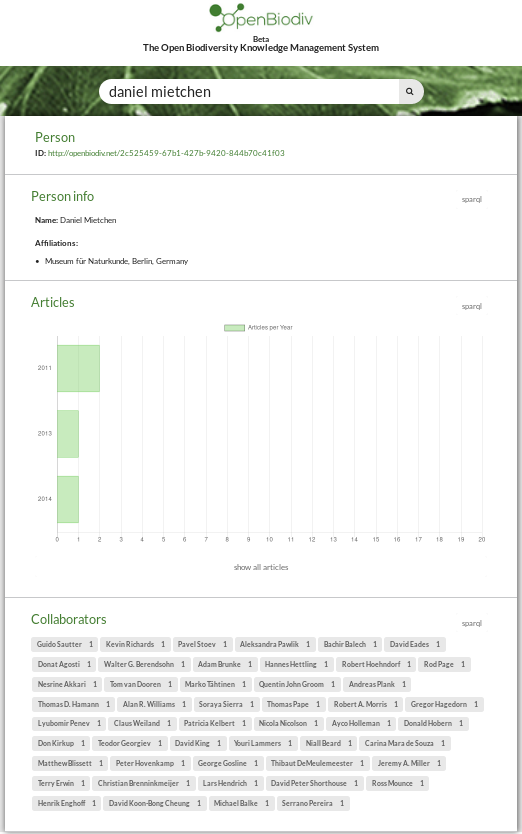
\includegraphics[width=\textwidth]{Figures/basic-level.png}
\decoRule
\label{fig:basic-level}
}
\end{frame}

\section{Обобщение}



\begin{frame}{Цел и задачи}

\begin{alertblock}{Цел}
Създаване на отворена система за информация за биоразнообразието, OpenBiodiv, основана на знание, извлечено от научната литература.
\end{alertblock}

\begin{block}{Задачи}
\begin{enumerate}

\item{Софтуерна архитектура} 

\item{Онтология на областта}

\item{Свързани отворени данни}

\item{Съпътвсваща софтуерна библиотека}

\item{Разработване на работни процеси}

\item{Уеб портал} 

\end{enumerate}
\end{block}
\end{frame}

\begin{frame}{Резултати}

\begin{enumerate}
    \item Софтуерна архитектура на OpenBiodiv (глава~1 и \cite{senderov_open_2016}).
    \item Концептуализация на областта на публикуването на знание за биоразнообразието във вид на онтологията OpenBiodiv-O (глава~2 и \cite{senderov_openbiodiv-o:_2018}). 
    \item Свързани отворени данни OpenBiodiv-LOD, под формата на RDF, обединяващи таксономично знание от Пенсофт, Плаци и GBIF (глава~3).
    \item Софтуерен пакет за манипулиране на RDF в средата за програмиране R, RDF4R (глава~4).
    \item Работен процес за автоматично вмъкване в онлайн ръкопис на данни от BOLD, GBIF, iDigBio, PlutoF. Автоматично създаване на онлайн ръкопис от EML файл с метаданни (глава~5 и \cite{senderov_online_2016}).
    \item Уеб сайт \href{http://openbiodiv.net}{openbiodiv.net} (глава~6).

\end{enumerate}

\end{frame}


\begin{frame}{Изпълнение на научната програма}

\alert{Смятаме, че постигнатите резултати удовляворат целта и задачите на докторантурата.} 

\end{frame}


\begin{frame}{Научни публикации}

\begingroup
\newcounter{count}
\setcounter{count}{99}
\defcounter{maxnames}{\value{count}}%

\begin{enumerate}
\item \longfullcite{senderov_open_2016} \alert{(най-малко 3 уникални цитата)}
\item \longfullcite{sarah_faulwetter_emodnet_2016}
\item \longfullcite{cardoso_species_2016} \alert{(най-малко 5 уникални цитата)}

\end{enumerate}

\endgroup

\end{frame}



\begin{frame}{Научни публикации}

\begingroup
\newcounter{count}
\setcounter{count}{99}
\defcounter{maxnames}{\value{count}}%

\begin{enumerate}
\setcounter{enumi}{3}
\item \longfullcite{senderov_online_2016} \alert{(най-малко 1 уникален цитат)}
\item \longfullcite{penev_strategies_2017} \alert{(най-малко 6 уникални цитата)}
\item \longfullcite{penev_arpha-biodiv:_2017} \alert{(най-малко 1 уникален цитат)}

\end{enumerate}

\endgroup

\end{frame}

\begin{frame}{Научни публикации}

\begingroup
\newcounter{count}
\setcounter{count}{99}
\defcounter{maxnames}{\value{count}}%

\begin{enumerate}
\setcounter{enumi}{6}

\item \longfullcite{arriaga-varela_review_2017} \alert{(импакт-фактор 1.031)}
\item \longfullcite{senderov_openbiodiv-o:_2018} \alert{(импакт-фактор 2.413, най-малко 3 уникални цитата)}
\end{enumerate}

\endgroup

\end{frame}


\begin{frame}{Journal of Biomedical Semantics}
\centering
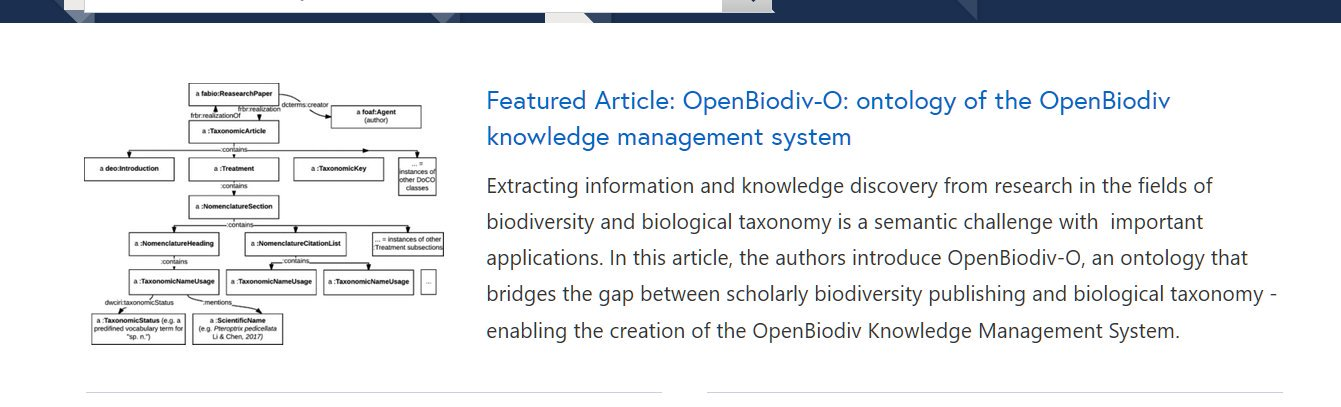
\includegraphics[width=\textwidth]{Figures/JBS-featured.jpg}
\decoRule
\\
\caption{Статията за OpenBiodiv-O е на началната страница JBS}
\label{fig:jbs-featured}
\end{frame}


\begin{frame}{Общо цитати}

\centering
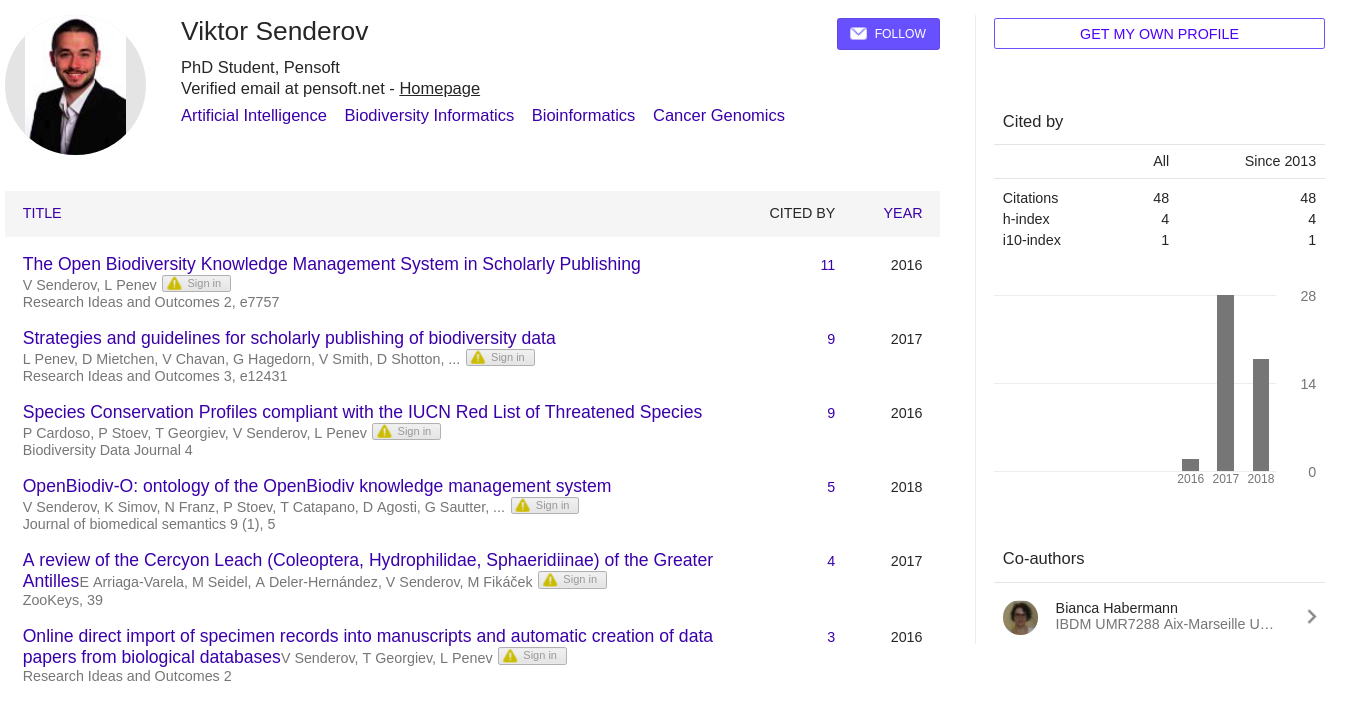
\includegraphics[width=\textwidth]{Figures/Google-scholar.png}

\end{frame}



\begin{frame}{Доклади пред научен семинар на ПНЗ}

\begin{enumerate}
    \item Доклад пред научен семинар на ИБЕИ на БАН на 26.10.2015 г. (``Публикуване, визуализация и разпространение на първични и геномни данни за биологичното разнообразие на основата на открита система за управление на информацията'').
    \item Доклад пред научен семинар в ИИКТ на БАН на 31.03.2016 г. (Open Biodiversity Knowledge Management System)
    \item Доклад пред научен семинар на ИИКТ на БАН за 23.03.2018 г. (OpenBiodiv: a knowledge-based system of biodiversity information)
\end{enumerate}

\end{frame}



\begin{frame}{Доклади пред международно научно мероприятие}

\begin{enumerate}
    \item Доклад пред международния симпозиум EU BON в София на 23.03.2016 г. (The Data Publishing Toolkit at EU BON: Automated creation of data papers, data and text integrated publishing via the ARPHA Publishing Platform.)
    \item Доклад по време на работната среща на BIG4 в Хавраники, Чехия на 03.06.2016 г. (Project Progress Report (OBKMS))
    \item Доклад по време на работната среща на BIG4 в Хавраники, Чехия на 03.06.2016 г. (Modern Methods of Systematic Research and the BOLD Algorithm)
    \item Уеб-базиран доклад (уебинар) пред международна аудитория в рамките на семинар на iDigBio на 16.07.2016 г. (Online direct import of specimen records from iDigBio instrastructure into taxonomic manuscripts)
    
    \end{enumerate}
\end{frame}


\begin{frame}{Доклади пред международно научно мероприятие}
\begin{enumerate}
\setcounter{enumi}{4}
    \item Доклад по време на работната среща на BIG4 в Копенхаген на 14.10.2016 г. (Midterm Progress Report)
    \item Доклад на международия симпозиум TDWG 2016 в Санта Клара де Сан Карлос от 5. до 9.12.2016 г. (Streamlining the Flow of Taxon Occurrence Data Between a Manuscript and Biological Databases)
    \item Доклад на международия симпозиум TDWG 2016 в Санта Клара де Сан Карлос от 5. до 9.12.2016 г. (The Open Biodiversity Knowledge Management System: A Semantic Suite Running on top of the Biodiversity Knowledge Graph)
    \item Доклад на международия симпозиум TDWG 2016 в Санта Клара де Сан Карлос от 5. до 9.12.2016 г. (Demonstrating the Prototype of the Open Biodiversity Knowledge Management System)
    \item Доклад на международия симпозиум TDWG 2016 в Санта Клара де Сан Карлос от 5. до 9.12.2016 г. (Creation of Data Paper Manuscripts from Ecological Metadata Language (EML))
   
\end{enumerate}
\end{frame}



\begin{frame}{Доклади пред международно научно мероприятие}
    \begin{enumerate}
    \setcounter{enumi}{9}
     \item Уеб-базиран доклад пред междуродния семинар на работната група по семантични технология към Университета Вандербилт (Тенеси, САЩ) на 20.02.2017 г. (Open Biodiversity Knowledge Management System)
    \item Доклад на европейската конференция на биосистематиците, BioSyst.eu 2016 на 15.08.2017 г. (The OpenBiodiv Knowledge System: The Future of Access to Biodiversity Knowledge)
    \item Доклад на международия симпозиум TDWG 2017 в Отава, Канада от 1. до 6.10.2017 г. (OpenBiodiv Computer Demo: an Implementation of a Semantic System Running on top of the Biodiversity Knowledge Graph)
    \item Доклад на международия симпозиум TDWG 2017 в Отава, Канада от 1. до 6.10.2017 г. (OpenBiodiv: an Implementaion of a Semantic System Running on top of the Biodiversity Knowledge Graph)
   
    \end{enumerate}
\end{frame}


\begin{frame}{Доклади пред международно научно мероприятие}
\begin{enumerate}
    \setcounter{enumi}{13}
     \item Постер на международия симпозиум TDWG 2017 в Отава, Канада от 1. до 6.10.2017 г. (OpenBiodiv: an Implementaion of a Semantic System Running on top of the Biodiversity Knowledge Graph)
    \item Доклад по време на работната среща на BIG4 в Ла Палма, Испания от 30. окт. до 3 ноем. 2017 г. (Midterm Progress Report)
    \item Доклад пред научен семинар на групата по биоинформатика (група Ронкуист) в Кралския природо-научен музей в Стокхолм на 29.11.2017 г.
\end{enumerate}
\end{frame}



\begin{frame}{Образователна програма}

\begin{enumerate}
    \item Изпит по базов специализиран предмет, проведен на 20.08.2018 г. Отл. (6). Комисия: проф. д-р Галя Ангелова, доц. д-р Кирил Симов
    \item Успешно положен изпит по езикова подготовка. (Изпит по английски език)   
    \item Успешно положен изпит по компютърни умения. (Изпит по програмиране с MATLAB)
    \item Курс ``Основи на таксономията и фаунистиката''. (Лектори: проф. Д.б.н. Бойко Б. Георгиев и Д-р Павел Н. Николов. Семестър: зимен семестър, 2015 г.)
 

\end{enumerate}

\end{frame}


\begin{frame}{Образователна програма}

\begin{enumerate}
    \setcounter{enumi}{4}
    \item Курс ``Увод в разнообразието и събирането на четирите големи групи насекоми'' от BIG4. Изследователска станция в Хавраники, Чехия. 4 - 11 юни 2016 г. Проф. Мартин Фикачек. Кредити по ECTS: 3.
    \item Курс ``Филогения, филогеномика, гражданска наука и предприемачество'' от BIG4. Изследователска станция в Туветорп, Швеция, 9 - 19 октомври 2016 г. Проф. Фредрик Ронкуист. ECTS: 4.
    \item Kурс ``Морфология на безгръбначните животни: 3D изображания и нови похвати в биосистематиката'' от BIG4. Природо-научен музей Виена, Австрия, 8 - 13 май 2017 г. д-р Несрин Акари. ECTS: 3.
    \item Kурс ``Историческа биогеография и диверсификационни анализи'' от BIG4. Ла Палма, Испания, 30 октомври - 3 ноември 2017 г. Проф. Никлас Валберг. ECTS: 1.5.

 

\end{enumerate}

\end{frame}

{
\setbeamercolor{background canvas}{bg=}

\includepdf[pages=14]{Figures/godishen-otchen-2017}
}



\section{Допълнителни слайдове}

\begin{frame}{Таксономични концепции}
\centering
  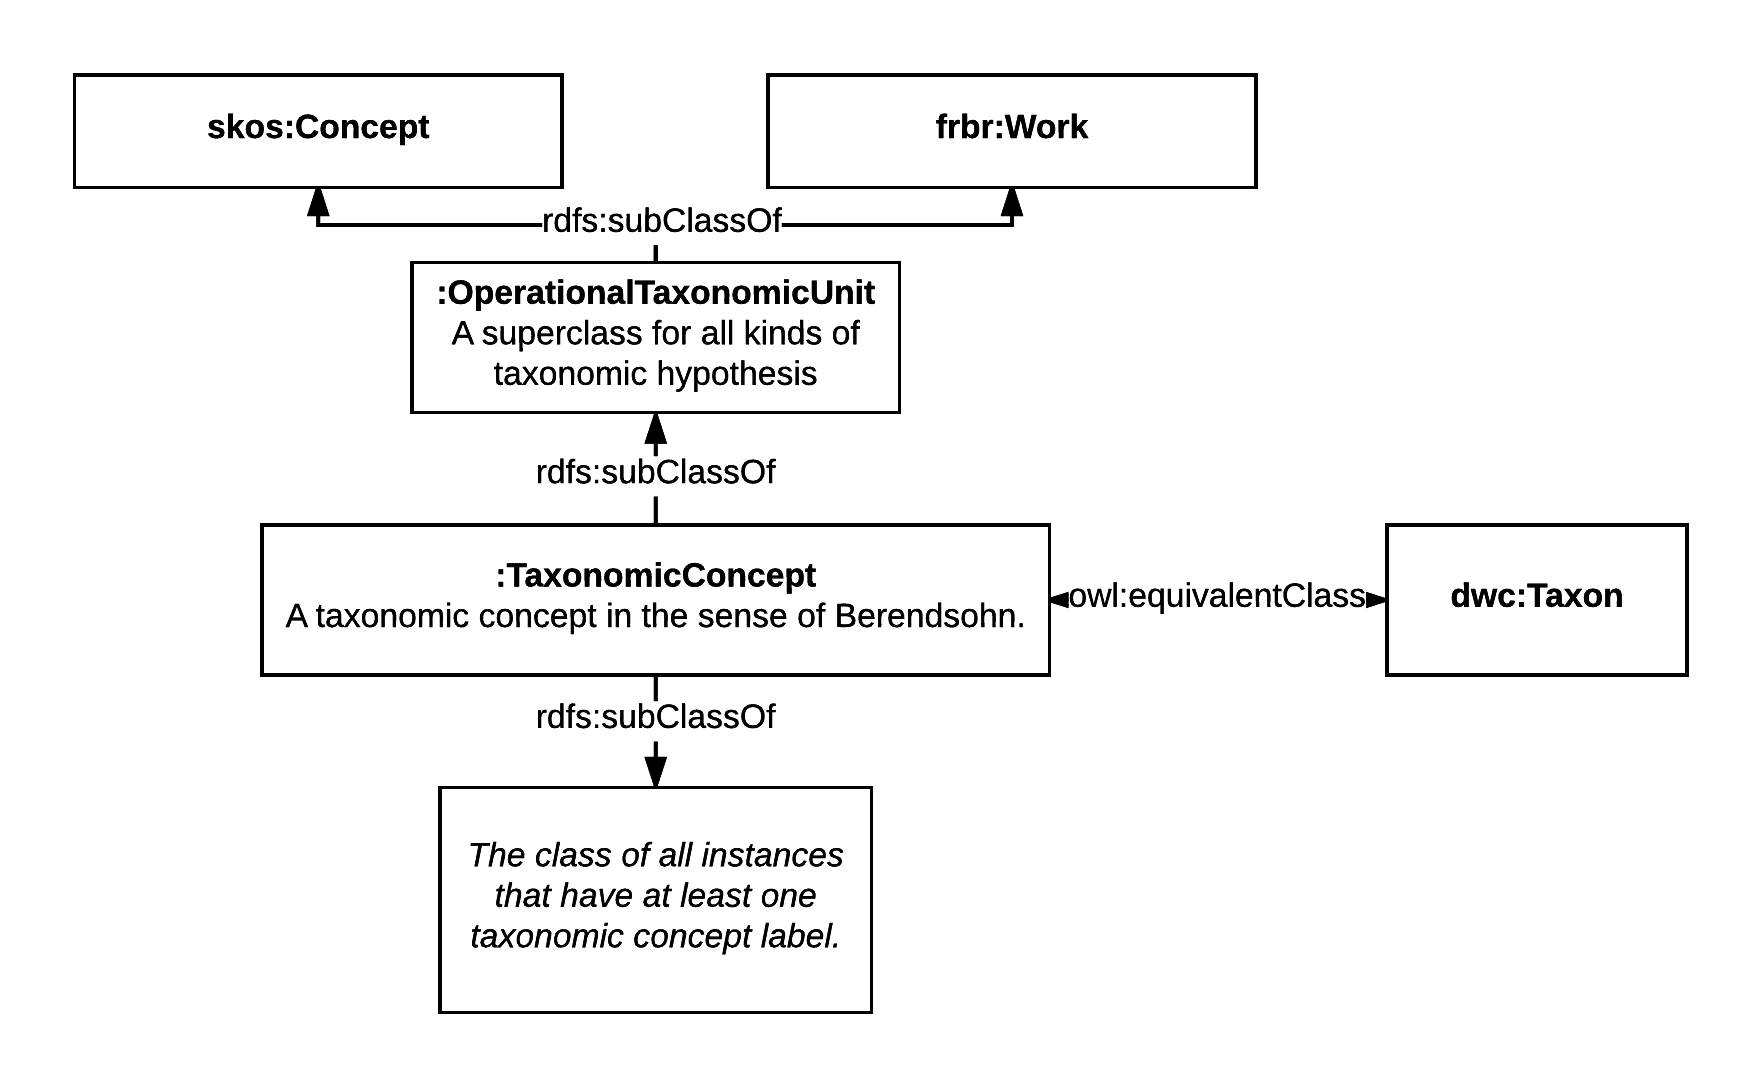
\includegraphics[width=\textwidth]{Figures/taxonomic-concept-diagram}
  \decoRule
  
\end{frame}


\begin{frame}{Example article metadata.}
	\centering

	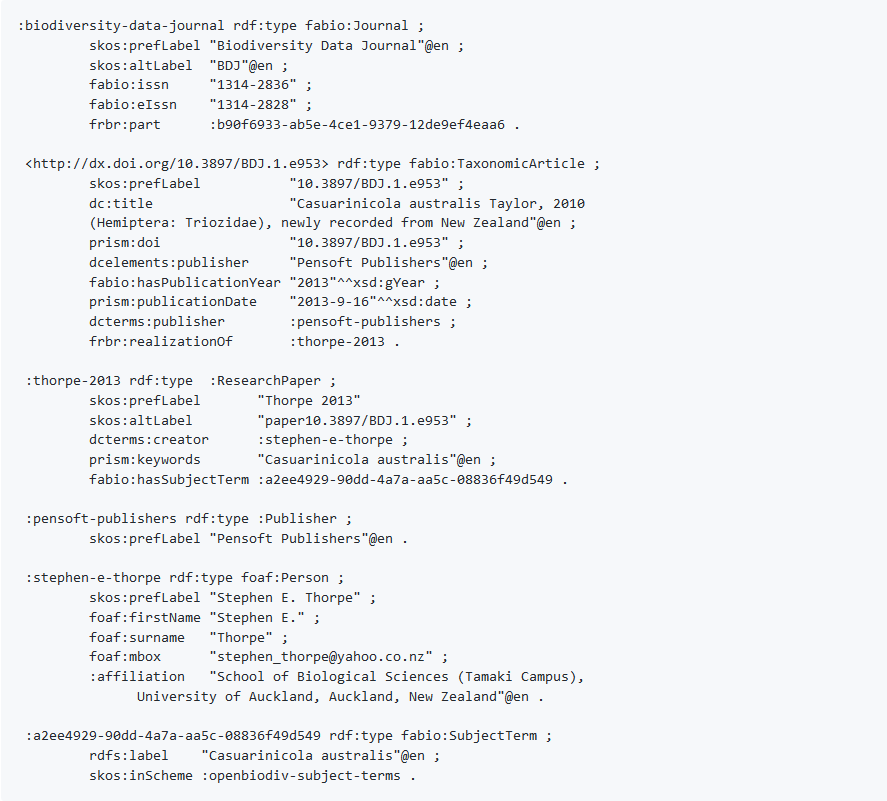
\includegraphics[width=\textwidth]{Figures/example-article-metadata}
	\decoRule
  
\end{frame}

\begin{frame}{Example article structure.}
  \centering
  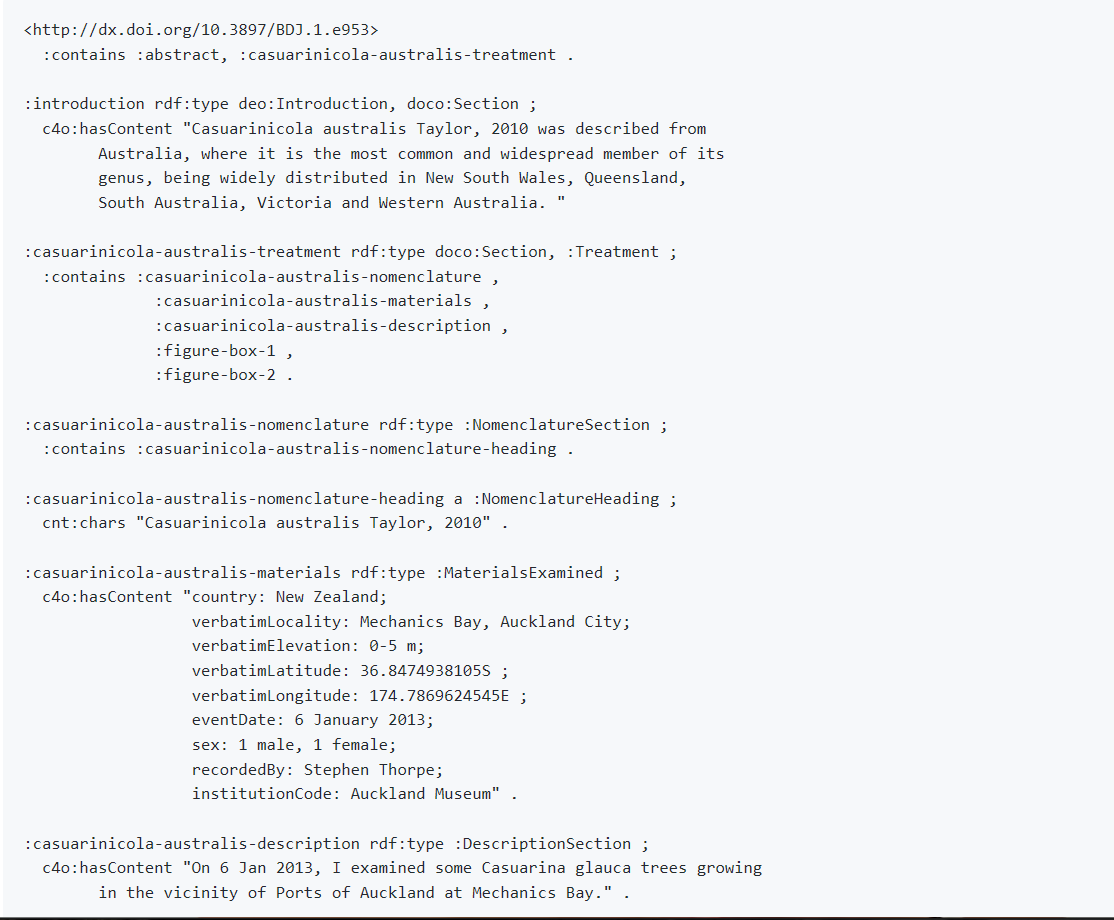
\includegraphics[width=\textwidth]{Figures/example-article-structure}
  \decoRule
\end{frame}

\end{document}